\chapter{Case Study I: Geo-diverse Data Centers}
\label{chap:casestudy1}
\section{Prelude}
Geo-diverse data centers enable robust and low-latency cloud services. The electricity cost for this huge infrastructure is a significant fraction of the operational cost (15\%)~\cite{costCloud} as well as capital cost~\cite{qureshiHotnets}. Due to increasing demand for cloud services and increasing electricity prices, it is essential for data center operators to cut their electricity bill~\cite{brill:DataCenterCrisis:UI:2007,Belady_EC_2007}.

In the previous chapter we presented an abstract and generalized electricity cost minimization framework that is applicable to geo-diverse data centers as well as cellular networks. In this chapter, we will derive a specialized instance of the general problem, discuss it's solution (exact as well as heuristic) and perform a sensitivity analysis.  We will also discuss our formulation's benefits and limitations.

The electricity cost savings resulting from workload relocation are somewhat limited due to lack of energy proportionality in today's data centers~\cite{10.1109/MC.2007.443}. Therefore, it was proposed to dynamically scale the active infrastructure in response to temporal variations in workload~\cite{10.1109/MC.2007.443,qureshi2009cutting}. This capacity scaling is expected to incur some overhead electricity cost which may be modeled as the \textit{state transition cost} in the state trajectory problem. 

Theoretically, one can benefit from capacity scaling by shutting down some equipment when it is not needed. However, some equipment in data centers may not be shut down because it is critical in nature. We term such equipment as inelastic load and the rest of the equipment as elastic load. Resource pruning of elastic load in data centers minimizes the electricity consumption, but conventional wisdom suggests that restarts affect equipment lifetime and operators are generally reluctant to adopt this approach. On the other extreme, elastic load may be left in an idle state, but the reduction in electricity  consumption would be quite small. In between these two extremes would be Dynamic Voltage and Frequency Scaling (DVFS) techniques. The transition cost would be zero for the idling scheme since no state-change overhead is incurred. The transition costs would be quite high if elastic load is de-activated (and activated later when needed), whereas DVFS would account for transition costs somewhere between the two extremes~\cite{Meisner:2009:PES:1508244.1508269}. In this thesis, we experiment with the entire spectrum of transition costs in order to generalize our results.

%The electricity load at a data center may be partitioned into two sets: one that is inelastic and must be on all the time and the other elastic portion that may be shutdown if there is no workload for the data center to handle. Let the first set comprise a fraction $r$ of the total data center power draw. The second part accordingly contributes a fraction $(1-r)$ of the total power draw. According to~\cite{Pelley:dcpower:weed:2009}, the breakup of power draw in a typical data center is servers: 56\%, cooling: 30\%, power conditioning: 8\%, network: 5\% and lighting: 1\%. Since we put only the servers in the elastic pool of devices, $r$ = 0.44. %In favor of ease of modeling, for most of the experiments discussed in our paper, we only put servers in the pool of elastic load. Some servers might need to always keep running, for instance, because they host critical services or in order to handle unexpectd traffic from end-hosts that have stale DNS or IP routing information. We expect these servers to contribute only a small amount of power consumption, in comparison to the pool of inelastic equipment and hence omitting this factor from the inelastic pool of equipment should not affect the results significantly. While airconditioning power draw is also somewhat load-dependent~\cite{Pelley:dcpower:weed:2009}, the assumption that airconditioning draws a constant amount of power irrespective of server status and workload does not favor the savings reported by our framework. A fraction of the power conditioning equipment that powers server may be shutdown along with the servers as needed, but the rest must stay on to keep the rest of the data center running. However, due to lack of statistics about the breakup of the power drawn by power conditioning equipment, we make the conservative assumption that all power conditioning equipment will keep running. Once again, this is an assumption that does not unduely favor the results of our framework. Shutting down networking equipment is expected to create undesirable transients in routing tables. Furthermore, if a small number of servers are required to always keep running, they will require layer-2 switches to be on as well. Hence, we place the network power draw completely in the inelastic pool. Placing lighting load in either pool should not create a significant deviation in the results. In our experiments, we take another conservative step by placing the lighting load in the inelastic pool.

\section{Related work}
To the best of our knowledge, prior work has largely taken a micro-scale view of this problem by scaling the data center capacity at the granularity of states of individual servers within a data center~\cite{Li:Optimal:TSG:2012,LinInfocom11,serverEnergy,Mazzucco2012415,rao2010,qureshi2009cutting} and, in some cases, has altogether ignored transition costs resulting from capacity scaling. These approaches lack scalability to multi-data center scenarios or are sub-optimal. In this thesis, we address the challenges of scalability as well as incorporation of transition costs into the optimization problem.

Li et. al. determined the electricity cost optimal mapping of workload to geo-diverse data centers by controlling the state of the individual servers within each data center~\cite{Li:Optimal:TSG:2012}. The state of the servers and their electricity consumption was controlled using Dynamic Voltage and Frequency Scaling (DVFS) and Dynamic Cluster Server Configuration (DCSC). Since their optimization problem formulation used Mixed Integer Programming (MIP) with decision variables per server, their approach is effective for small-scale problems such as an individual data center or a fraction thereof. This limitation is evident from the small number of servers used in the simulation-based evaluation in~\cite{Li:Optimal:TSG:2012}. One way to scale their approach to large distributed data centers is to use coarse granularity in their problem formulation. For instance, instead of controlling the state of each server independently, all servers in a single rack could be configured in the same state at a given time. They used the Soccer World Cup 1998 webserver workload traces and electricity prices at four different locations to evaluate their proposal. 

Some researchers have also proposed algorithms for the data center electricity cost optimization problem. In the context of a web-search query processing system hosted on a geo-diverse data center network, Kayaaslan et. al. presented a bin-packing type of algorithm for shifting search query workload between data centers in~\cite{Kayaaslan:2011:EQP:2009916.2010047}. Buchbinder et. al. proposed online algorithms for relocating Map Reduce jobs between geo-diverse data centers to reduce the electricity bill while considering the cost of inter-data center bandwidth~\cite{Buchbinder:2011:OJR:2008780.2008798}. Their proposed algorithms consider the uncertainty in electricity prices and workload estimates while mapping the jobs to data centers. They evaluated their algorithms using electricity prices from $30$ locations across the US and workload data from a $10000$ node Map Reduce cluster. Bhaskar et. al. proposed online algorithms for mixed packing and covering, a problem which may be applied to optimally map workload to geo-diverse data centers~\cite{Bhaskar:2012:CoRR}. For configuring servers in a single data center with a view of minimizing electricity costs, Lin et. al. presented offline as well as online algorithms for dynamic scaling of server computational capacity~\cite{LinInfocom11}. Urgaonkar et. al. proposed an online optimization algorithm while proposing to disconnect data center devices from mains and running on UPS when the electricity prices are high~\cite{Urgaonkar:2011:OPC:1993744.1993766}. Their proposed scheme recharges the UPS units when the electricity prices are lower.

Investigations of infrastructure scaling strategies to conserve power in a single data center are reported in~\cite{serverEnergy,Mazzucco:Maximizing:2011:CoRR,Oh:2011:ECS:2170444.2170458,Chase:2001:MES:502059.502045}. Chen et. al. proposed three different solutions that either shut down or frequency-scale servers in a web hosting data center with the objective of minimizing electricity and maintenance cost while ensuring SLA compliance~\cite{serverEnergy}. The first two of the proposed algorithms were based on a queuing theoretic and control theoretic analysis, respectively, while the third one was a hybrid scheme. While scaling the deployed capacity, their proposed scheme considers the cost of turning the servers on and off in terms of the resulting wear and tear. Mazzucco et. al. presented similar strategies in~\cite{Mazzucco:Maximizing:2011:CoRR}. Oh et. al. considered a virtualized environment and proposed solutions for optimally placing VMs on servers and map workload to the VMs such that electricity costs are minimized~\cite{Oh:2011:ECS:2170444.2170458}. In~\cite{Chase:2001:MES:502059.502045}, Chase et. al. presented policies for resource allocation in a hosting center alongwith a switching infrastructure for routing requests to servers.

Most of the prior work in this area considers applications with short request-response type jobs. In~\cite{Chen:2008:ESP:1387589.1387613}, however, Chen et. al. considered connection-intensive applications such as video streaming, Internet gaming and instant messaging in the context of energy cost aware load dispatch. 

Rao et. al. consider data center operation in a futures electricity market and the possibility of hedging against uncertain electricity prices under a smart grid environment in~\cite{Rao:2011:TSG}. The authors used workload data from Google search cluster and evaluated a scenario of an operator with data centers at two different locations.

Another related theme of research is greening of data centers. Some examples of work that reports the results of efforts towards \textit{green} mapping of workload to data centers are:~\cite{Le:HotPower:2009,Zheng2011275,Koutitas:2010:JGE,abbasi2011dahm,chiaraviglio2010greencoop,Phan:2012:GECCO,Liu:2011:SIGMETRICS,Liu:2011:GREENMETRICS}. On a related note, Sucevic et. al. studied various approaches for shutting down end-hosts to minimize the total electricity consumption on participant hosts in a peer-to-peer file download system~\cite{Sucevic:2011:PDE:2160803.2160864}.

All of the above work deals with problems that can be categorized broadly as optimal scheduling problems. Such problems arise in many different domains and prior work in such domains is relevant. For instance, System on Chip (SOC)~\cite{Fang:2011:COP:1995896.1995940}, electric power systems and smart grid~\cite{Javed:2008:ULP:1485753.1485792,Logenthiran2011138,Celli:2001:PICA,FahadJavedAdOpt.SASO.2009.26}, WiFi access points~\cite{Marsan:2010:SAM:1791314.1791340}, wide area networks~\cite{Cavdar:2011:ECOC}, cellular networks~\cite{Peng:2011:TPS:2030613.2030628} and high performance computing~\cite{Lee:ServerConsolidation:2011:Globecom,Pinheiro01loadbalancing,Yao:DCPowerReduction:2012:INFOCOM,Herodotou:Starfish:2011:CIDR,Herodotou:2011:NOS:2038916.2038934,Aikema:ElecCostHPC:2011:ISSST}.

\section{Instantiating the generalized optimization formulation}\label{sec:case1:instantiating} %Derive the objective function and constraints. Clearly outline the assumptions that we've made about the geo-diverse data centers.
Consider a geo-distributed data center infrastructure
comprising $m$ interconnected data
centers. At any given time, the workload is distributed amongst the data
centers in the network. For ease of modeling, we assume that changes to the distribution of workload amongst data centers may be done at the start of discrete intervals of duration $\lambda$. We use $x_i^j$ to denote the fraction of workload during interval $j$ that is mapped to data center $i$.  We consider workload that is normalized over it's peak, i.e., the workload values for any interval are between 0 and 1. The workload capacity of data center $i$, denoted $c_i$, is also normalized on the same scale. We assume that the network of data centers is over-subscribed so that $\sum_{i=1}^m c_i > 1$.

Let the sum of elastic load's peak and idle power consumption over all data centers be $P^{max}$ and $P^{min}$, respectively. Assuming that the data centers are homogenous, an individual data center's workload capacity is directly related to it's peak (or idle) power consumption. Thus, $P_i^{max} = c_iP^{max}$ and $P_i^{min} = c_iP^{min}$. 

Data center power consumption is an affine function of the average CPU utilization of the servers~\cite{Fan:power:ICSA:2007}. Therefore, the average power consumption at data center $i$ during interval $j$ is: 
\begin{align}
P_i^j = c_i \left(P^{min}+\frac{x_i^j\left(P^{max}-P^{min}\right)}{c_i}\right)
\end{align}
Dividing both sides of the above equation by $P^{max}$ gives the normalized power consumption for data center $i$ during interval $j$:

\begin{align}
\label{eq:dcpower}
\hat{P_i^j} = fc_i + x_i^j\left(1-f\right)
\end{align}
where $f$ is the ratio of $P^{max}$ to $P^{min}$. If we set $x_i^j=0$, i.e., data center $i$ is not computing any workload during interval $j$, then the second term in equation~\ref{eq:dcpower} goes to zero and the power consumption reduces to the first term in equation~\ref{eq:dcpower} only, which we refer to as \textit{idle power consumption}. The second term in equation~\ref{eq:dcpower} indicates the workload-dependent \textit{computational power consumption}, which is independent of the data center capacity.

Let $\sigma$ and $\delta$ be the average power consumption, over a single interval, required to activate or deactivate, respectively, all of the elastic load at a unit capacity data center. Then, the power consumption for activation of the elastic load at data center $i$ is $\sigma c_i$. The electricity cost for activating data center $i$'s elastic load at the start of interval $j$ is, therefore\footnote{Multiplication with the duration of an interval, i.e., $\lambda$ is not necessary, because $\sigma$ is defined as the per interval cost.}, $c_ie_i^j\sigma$. Here, we are assuming that the elastic load at a data center may be activated within a single interval. The value of $\lambda$ that we used in our experiments is equal to one hour, which is a sufficiently large interval for server activation. Deactivation cost for elastic load may also be derived in a similar manner. 

Electricity cost incurred at data center $i$ during interval $j$ is a product of it's total power consumption (computing, idling, activation and deactivation), duration of the interval ($\lambda$) and the unit price of electricity ($e_i^j$). Hence, the RED-BL optimization problem formulation may be given as:

\begin{align}
\text{minimize } \sum_{j=1}^{n} \sum_{i=1}^{m} c_i e_i^j\left(p_i^j \lambda\left(f+\left(1-f\right)\frac{x_i^j}{c_i}\right) + b_i^j \sigma + s_i^j \delta\right) \label{eq:objective}
\end{align}
subject to:
\begin{align}
x_i^j \le c_i \hspace{6 pt} \forall i, \forall j \label{eq:capcon}\\
\sum_{i = 1}^{m} x_i^j = w^j \hspace{6 pt} \forall j \label{eq:workcon}\\
p_i^j, b_i^j, s_i^j \in \{0,1\} \hspace{6 pt} \forall i, \forall j \label{eq:integer1}\\
p_i^j \ge x_i^j \hspace{6 pt} \forall i, \forall j \label{eq:p1}\\
b_i^j \ge p_i^j - p_i^{j-1} \hspace{6 pt} \forall i, 2 \le j \le n \label{eq:bcon}\\
%\end{align}
%\begin{align}
s_i^j \ge p_i^{j-1} - p_i^j \hspace{6 pt} \forall i, 2 \le j \le n \label{eq:scon}\\
b_i^0 = p_i^0, s_i^0 = 0 \hspace{6 pt} \forall i \label{eq:bcon1}
\end{align}

\begin{table}
\begin{center}
\begin{tabular}{cl}
\hline Parameter & Description \\
\hline $m$ & Number of data centers \\
%$r$ & Fraction of data center load that is inelastic, i.e., may never be shutdown \\
 $n$ & Number of intervals in a planning window \\
 $\lambda$ & Duration of an interval in hours \\
  $f$ & The ratio between a data center's peak and idle power consumption \\
 $c_i$ & Normalized workload capacity of data center $i$ \\
 $\sigma$ & Penalty for activating the elastic load at a unit capacity data center as a fraction\\
\ & of its energy consumption at full load in one interval \\
 $\delta$ & Penalty for deactivating the elastic load at a unit capacity data center as a fraction\\
\ & of its energy consumption at full load in one interval \\
 $e_i^j$ & Unit cost of electricity at data center $i$ during interval $j$ \\
 $w^j$ & Operator's workload during interval $j$ \\
 $x_i^j$ & Workload mapped to data center $i$ during interval $j$ \\
 $p_i^j$ & 1 if data center $i$ is active (either computing workload or\\
\ & idling) during interval $j$, $0$ otherwise \\
 $b_i^j$ & 1 if data center $i$'s elastic load is activated at interval $j$, $0$ otherwise \\
 $s_i^j$ & 1 if data center $i$'s elastic load is deactivated at interval $j$, $0$ otherwise \\
\hline
\end{tabular}
\caption{Data Center Network Model Parameters}
\label{tab:model}
\end{center}
\end{table}

Decision variable $p_i^j$ is 1 if the elastic load in data center $i$ is active during interval $j$, or 0 otherwise. Similarly, $b_i^j$ ($s_i^j$) is 1 if the elastic load in data center $i$ is activated (deactivated) at the start of interval $j$. In equation~\eqref{eq:objective}, multiplication of the first two terms by $p_i^j$ ensures that computation and idling costs are accounted for in interval $j$, only if the elastic load in data center $i$ is active during that interval. Similarly, multiplication of the last two terms in equation~\eqref{eq:objective} by $b_i^j$ and $s_i^j$, respectively, ensures that activation and de-activation costs contribute to the summation only when the elastic load in a data center is activated or de-activated.

The workload capacity constraint is given in~\eqref{eq:capcon}. Eq.~\eqref{eq:workcon} ensures that all incident workload is handled, while~\eqref{eq:integer1} represents the binary-value
constraint. Inequality~\eqref{eq:p1} ensures that the elastic load in a data center
is active whenever there is any workload mapped to it. The constraint in Eq.~\eqref{eq:bcon} ensures that $b_i^j$ is 1 if the elastic load is inactive in interval $j-1$ and active in the next interval. The involvement of $b_i^j$ in the minimization objective function ensures that it is 0 otherwise. Similarly, the constraint in Eq.~\eqref{eq:scon} ensures that $s_i^j$ takes on the correct value depending on the deactivation of elastic load in the data centers. We assume that the elastic load in all data centers is initially inactive, therefore, an activation may be necessary at the first interval whereas deactivation in the first interval is not necessary. These conditions are ensured by the constraints in Eq.~\eqref{eq:bcon1}. It is easy to customize this constraint such that all data centers are assumed to be initially active.

\section{Sources of transition costs in the data center scenario}
This thesis uses the overhead of data center activation/deactivation as the transition costs. However, in practice, there can be other forms
of transition costs as well, which would vary from one deployment to the other. Examples of other sources of transition costs include, but may not be limited to, the following:

\begin{itemize}
\item An operator might change the way user traffic is
    routed to data centers by modifying entries in the
    Domain Name System (DNS). In such cases, it has been
    reported that many client-side DNS caches violate the
    DNS entry Time-To-Live (TTL) by continuing to cache
    expired DNS entries~\cite{Pang_IMC_2004}. This means
    that user traffic may continue to arrive at a data
    center that the operator does not intend to handle
    workload at. If this overwhelms the active data center capacity, it may result in lost revenue due to excessive response times.
\item The operator might change the way user traffic is
    routed to data centers by making changes to the Border
    Gateway Protocol (BGP) routing table. Due to the
    complex nature of inter-service provider connectivity
    and BGP dynamics, BGP routing table changes have been
    shown to take an unpredictable amount of time to
    reflect globally~\cite{LabovitzSigcomm}. This means
    that we run into a similar situation as for the
    DNS-based method described above.
\item In order for any request to be handled anywhere, the
    data store for the applications must be replicated and
    consistency must be maintained.  The cost of inter-data center traffic is quite high, hence this form of transition costs would be quite significant. The magnitude is not easy to predict because replication schemes are operator and
    application dependent. To the best of our knowledge, the current body
of knowledge lacks a generic model for such traffic. Therefore, similar to~\cite{qureshi2009cutting}, in this thesis, we assume
that content is perfectly replicated.
\end{itemize}

It is clear from the above discussion that the factors contributing towards
transition costs depend not only on how the data center network
is deployed and operated but also on the applications being
hosted. Since this information is confidential, the utility of
modeling a specific deployment is limited. The question that is
significant, however, is the impact on the possible electricity
cost savings (resulting from geo-temporal diversity in
electricity prices) of variation in the magnitude of transition
costs relative to the electricity cost in a given interval. Therefore, we have used a normalized and parametrized model for transition costs in our problem formulation. Our aim in this thesis is to present
electricity cost optimization solutions which operators can
use, along with the parameter data (idling costs, transition
costs, number of data centers and their locations) from their
own data center network.

\subsection{Problem complexity and a heuristic}
\label{subsec:complexityheur}The optimal workload relocation problem is identical to the Unit-Commit problem~\cite{unitcommit-trans} in distributed
electricity generation and transmission scenario. In the unit
commit problem, one determines the amount of power to be supplied from each generating resource and schedules the activation (ramp up), deactivation (ramp down) and idling (spinning reserves) of the generating resources, given time-varying demand for
electricity. Due to a one-to-one mapping between the data center-workload mapping and Unit-Commit problems, it follows that if there is a polynomial time solution for the data center-workload mapping problem, Unit-Commit may also be solved in polynomial time. However, since the Unit-Commit
problem is known to be NP-Complete~\cite{unitcommit-trans}, it follows that so is the
workload-mapping problem that we are considering in this thesis.
We will show later that we are able to solve reasonably large sized instances of the above NP-Hard MIP formulation for RED-BL using the CPLEX solver. Nonetheless, we now present a heuristic algorithm for it.

The pseudo-code of our heuristic algorithm for RED-BL is given in Algorithm~\ref{algo:heur1}. Assume that the workload vector for the planning window starts at a trough, then rises in a non-decreasing manner to the peak before falling off in a non-increasing manner to another trough. Since the activation/deactivation costs are expected to be significant, our heuristic is designed to select a small number of data centers to operate in long continuous stretches during a given day. For the assumed characterization of the workload, elastic load at a few data centers would be sufficient to handle the workload early (and late) in the planning window. As the workload rises gradually, elastic load at some more data centers would need to be brought online. As the workload starts to fall, elastic load at some data centers may gradually be deactivated until the planning window ends. Our heuristic places two pointers at the beginning and end of the planning window, determines the number of data centers ($d_1$ and $d_2$) needed to handle the workload corresponding to the two pointers and picks the smaller of these two values. It then finds min($d_1$, $d_2$) best data centers in terms of having the least average electricity price over the planning window. The elastic load at these data centers will be kept active between the intervals corresponding to the two pointers. Furthermore, our algorithm assigns as much workload as possible to the selected data centers in ascending order of average electricity price in the chosen intervals. 

As long as the workload in the intervals corresponding to the two pointers may be handled by the same number of data centers, both of the pointers are moved closer to each other. Otherwise, the pointer that corresponds to the interval requiring the smaller number of data centers is moved towards the other pointer. This pointer movement is performed until either the pointers cross each other or the number of data centers required to handle the workload in the interval corresponding to the moving pointer increases. In the former case, we are done and in the latter, the algorithm repeats the data center selection and workload mapping step. The algorithm then activates elastic load at data center(s) to meet the workload requirement of the pointer corresponding to the interval with the higher workload. The data center(s) where the elastic load is activated at this time are the ones that are not used before and have the least average electricity price in the interval between the two pointers.

\begin{algorithm}
\caption{Heuristic for the RED-BL problem}
\label{algo:heur1}
\begin{algorithmic}[1]
\REQUIRE $w[1..n]$: Cumulative data center workload for the planning window,\\$e[1..m][1..n]$: Electricity prices for all data centers over the planning window
\ENSURE $z[1..m][1..n]$: workload assigned to the data centers for all intervals\\
$y[1..m][1..n]$: Data center status (1=on/0=off) over the planning window
\STATE $g_1 = 0$; \quad $g_2 = n-1$; \quad $l = w$; \quad $a = 1..m$; \quad $n_c = 0$;
\STATE \quad $y[i][j]=0$; \quad $z[i][j]=0$; \quad ($\forall i, \quad \forall j$)
\REPEAT
	\STATE $d_1 = \lceil w[g_1]/c_1 \rceil$; \quad $d_2 = \lceil w[g_2]/c_1 \rceil$; \quad $n_d = \min(d_1, d_2)$
	\IF{$n_d > n_c$}
		\STATE Sort $a$ in ascending order of average electricity price in $[g_1, g_2]$
		\FORALL{$i \in a$}
			\FORALL{$j \in [g_1, g_2]$}
				\STATE $y[i][j] = 1; \quad n_c$++
				\STATE $z[i][j]=\min(l[j], c_i)$
				\STATE $l[j] = l[j] - z[i][j]$				
				\STATE Remove $i$ from $a$
			\ENDFOR
		\ENDFOR
	\ENDIF
		\REPEAT
			\STATE $g_1$++
		\UNTIL{$(\lceil w[g_1]/c_1\rceil > n_c) \OR (g_1 > g_2) \OR (\lceil w[g_1]/c_1\rceil > \lceil w[g_2]/c_1\rceil)$}
		\REPEAT
			\STATE $g_2$- -
		\UNTIL{$(\lceil w[g_2]/c_1\rceil > n_c) \OR (g_1 > g_2) \OR (\lceil w[g_1]/c_1\rceil < \lceil w[g_2]/c_1\rceil)$}
\UNTIL{$g_1 > g_2$}
\end{algorithmic}
\end{algorithm}


On line 1, the algorithm starts by placing two pointers, $g_1$ and $g_2$, at the extremes of the workload vector. Our algorithm would work best if the beginning and end of the workload vector conincides with the two troughs of the workload in the planning window. Also, on line 1, our algorithm makes a local copy $l$ of the workload vector $w$, so that $l$ may be used to keep track of the algorithm's progress without modifying the input vector. Line 1 also includes the initialization of a list of available data center indices, $a$, and the initialization of the number of data centers currently in use, $n_c$, to zero. These steps would run in O($m$+$n$).

The algorithm will store it's solution in 2-D arrays $y$ and $z$. Here, $y[i][j]$ is 1 if data center $i$ is to be on during interval $j$ and 0 otherwise. Furthermore, $z[i][j]$ holds the amount of workload to be mapped to data center $i$ during interval $j$. This initialization takes O(m$n$).

The algorithm starts by computing the minimum number of data centers required to handle the workload during intervals $g_1$ and $g_2$ as the values $d_1$ and $d_2$, respectively. Since we have considered homogenous data centers, all $c_i$ are equal, therefore, this computation uses $c_1$ as the capacity of a data center. The smaller of $d_1$ and $d_2$ is picked as $n_d$. If $n_d$, the minimum data center demand during [$g_1, g_2$] is greater than the current number of active data centers $n_c$, the algorithm enters the if-block on line 6. On line 7, the algorithm first computes the average electricity price for the available data centers between intervals $g_1$ and $g_2$ in O(m$n$) and then sorts the available data center indices in ascending order of average electricity price from $g_1$ to $g_2$ in O(m lg m). Between lines 8 and 15, the algorithm marks $n_d - n_c$ data centers to be on from $g_1$ to $g_2$ (line 10), updates the current number of data centers that have been used by the algorithm, $n_c$ (line 10), assigns workload to each of these data centers (line 11), updates the local copy of the workload vector, $l$, by subctracting the amount of workload  that the algorithm has handled so far for the relevant intervals and removes the data centers that have been assigned workload from the list of available data center $a$ (line 13). Since line 13 involves removal of some contiguous entries from the beginning of an array, it runs in O(m).

Lines 17-22 update the two pointers until they either demark a section of the workload vector that requires a greater number of data centers than $n_c$ or $g_1$ exceeds $g_2$ (which means that we are done). If the workload during intervals $g_1$ and $g_2$ is such that they both require the same number of data centers, both of the repeat until loops run and pointers $g_1$ and $g_2$ are moved until they reach a point where the workload for each pointer requires a greater number of data centers. Otherwise, only one of the repeat-until loops runs and the pointer corresponding to the interval requiring the smaller number of data centers is moved towards the other pointer until it reaches an interval where the workload requires a greater number of data centers.

The if-block (line 6-16) will dominate the overall execution time. Within this if-statement, on line 7, the average electricity price is computed and then the data center indices are sorted in ascending order. In the worst case, the if-block will be entered in every iteration of the outer repeat-until loop and exactly one data center index will be removed from $a$ (line 13) in each iteration of the outer repeat-until loop. In this case, the computation of average electricity prices will require m$n$ + (m-1)($n$-1) + (m-2)($n$-2) + (m-3)($n$-3) + ... + (m-$n$+1) primitive operations. Sorting the electricity prices will require O(m lg m) + O((m-1) lg (m-1)) +  ... + O((m-$n$+1) lg (m-$n$+1)) running time, overall. Within the nested for-loops, line 13 is most complex which will require, in the worst case, (m-1) + (m-2) + (m-3) + ... + (m-$n$-1) primitive operations. This is smaller compared to the running time of the average electricity price computation, so in Big-Oh notation, we can ignore it. The overall worst case running time for the electricity price averaging can be computed as follows. We first consider that the electricity price averaging is done exactly $i$ times and will later replace $i$ by it's actual value of $n$.

\begin{align}
mn + \left(m-1\right) \left(n-1\right) + \left(m-2\right) \left(n-2\right) + ... + \left(m-i+1\right) \left(n-i+1\right)\notag \\
i mn - n - 2n - ... - \left(i-1\right)n - m - 2m - ... - \left(i-1\right)m + 1 + 4 + ... + \left(i-1\right)^2\notag \\
i m n - \left(n + m\right)\left(1 + 2 + ... + \left(i-1\right)\right) + 1 + 4 + ... + \left(i-1\right)^2\notag \\
i mn - \left(n + m\right)\frac{i\left(i+1\right)}{2} + \frac{n\left(n-1\right)\left(2n-1\right)}{6}\notag
\end{align}
Substituting $i$ by $n$, we get the overall worst case running time for the average electricity price calculation step as O(m$n^2$ + $n^3$). The overall worst case running time of the entire algorithm (including the average electriciry price sorting step) is O(m$n^2$ + $n^3$ + m lg m).

In the best case, only one data center is sufficient to handle all workload throughout the planning window and the outer repeat-until loop is only entered once. The average electricity cost is computed in O(mn), and the data center indices are sorted in O(m lg m). Removal of the sole selected data center's index from the array of available data center indices is done in O(m), whereas the increment of $g_1$ and decrement of $g_2$ is O(n). Hence, the best case running time complexity of the algorithm is O(mn + m lg m).

%
%Figure~\ref{fig:heur1perf} shows the performance of the heuristic compared to the optimal solution of the problem for various values of the (de)activation overhead parameters. For each value of the $b$/$s$ parameters, we have plotted the average error over the seven days in our workload dataset (the curve) as well as the minimum and maximum error for any given day (the vertical bars). The performance of the heuristic is the worst for $b$/$s$ = 0, because the heuristic avoids bootup/shutdown which has zero cost for $b$/$s$ = 0. For other small values of $b$/$s$ also, the bootup/shutdown overhead is not significant and by avoiding it, our heuristic fares relatively poorly compared to the optimal solution. As the value of $b$/$s$ increases, our heuristic's error compared to the optimal solution drops until it starts a slight rise. The rising trend in the heuristic's performance for relatively high values of $b$/$s$ is because in this regime, it may often be better to allow idling of some data centers instead of a bootup at the intervals defined by $g_1$ and shutdown at those defined by $g_2$. We observed similar trends for other values of $f$ as well, when $b$/$s$ is varied from 0 to 1.
%
%\begin{figure}
%\includegraphics[width=1\linewidth]{../Matlab/rb-heur1error.eps}
%\caption{Heuristic 1 performance}
%\label{fig:heur1perf}
%\end{figure}

\section{Experimental setup}
\label{sec:experiments} 
In this section, we describe the experimental setup to perform a comparative study of different workload placement algorithms under various scenarios.

\subsection{Application workload}
We used an year-long trace of hourly workload for $3$ social networking applications, with a subscription base of over $8$ million users~\cite{Nazir:2008:UFM:1452520.1452527}. In order to make the dataset representative of a large data center network operator, we aggregated these traces into a week long trace as follows. We sliced the trace into week-long segments and considered each slice as workload for a different application, for the same week. We, then, normalized the sum of these trace vectors so that the peak cumulative workload corresponds to a value of $0.9$. The normalized workload intensity is plotted in Figure~\ref{fig:workloadr}. The statistical characteristics of our workload, as plotted in Figure~\ref{fig:workloadhist} are quite similar to those reported by Google for ``thousands of servers during a six-month interval at a Google data center"~\cite{10.1109/MC.2007.443}.

\begin{figure}%[htbp]
  \begin{minipage}[b]{0.5\linewidth}
    \centering
    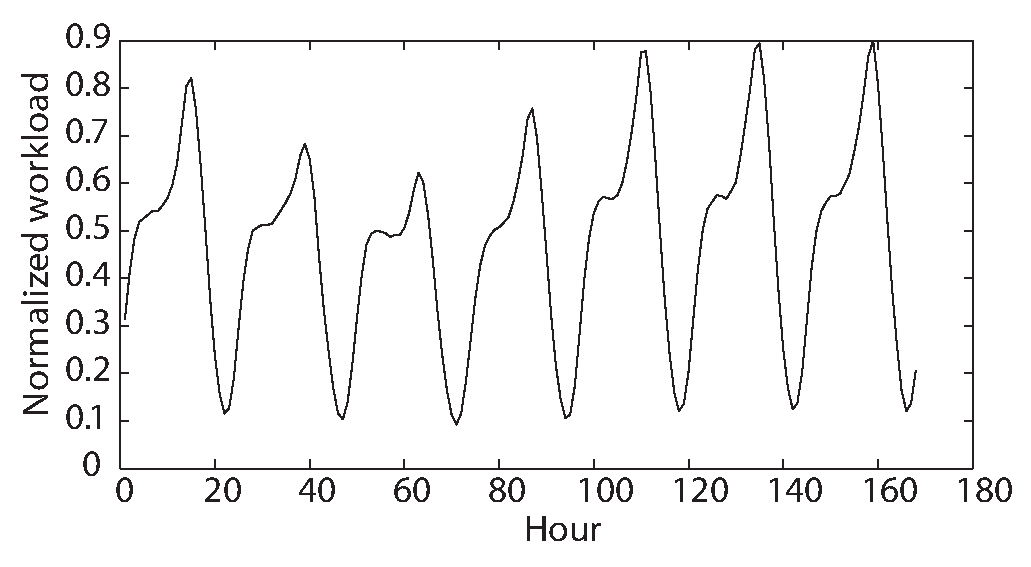
\includegraphics[width=\linewidth]{pics/workloadr.eps}
    \caption{Normalized workload}
    \label{fig:workloadr}
  \end{minipage}
  \hspace{0.5cm}
  \begin{minipage}[b]{0.5\linewidth}
    \centering
    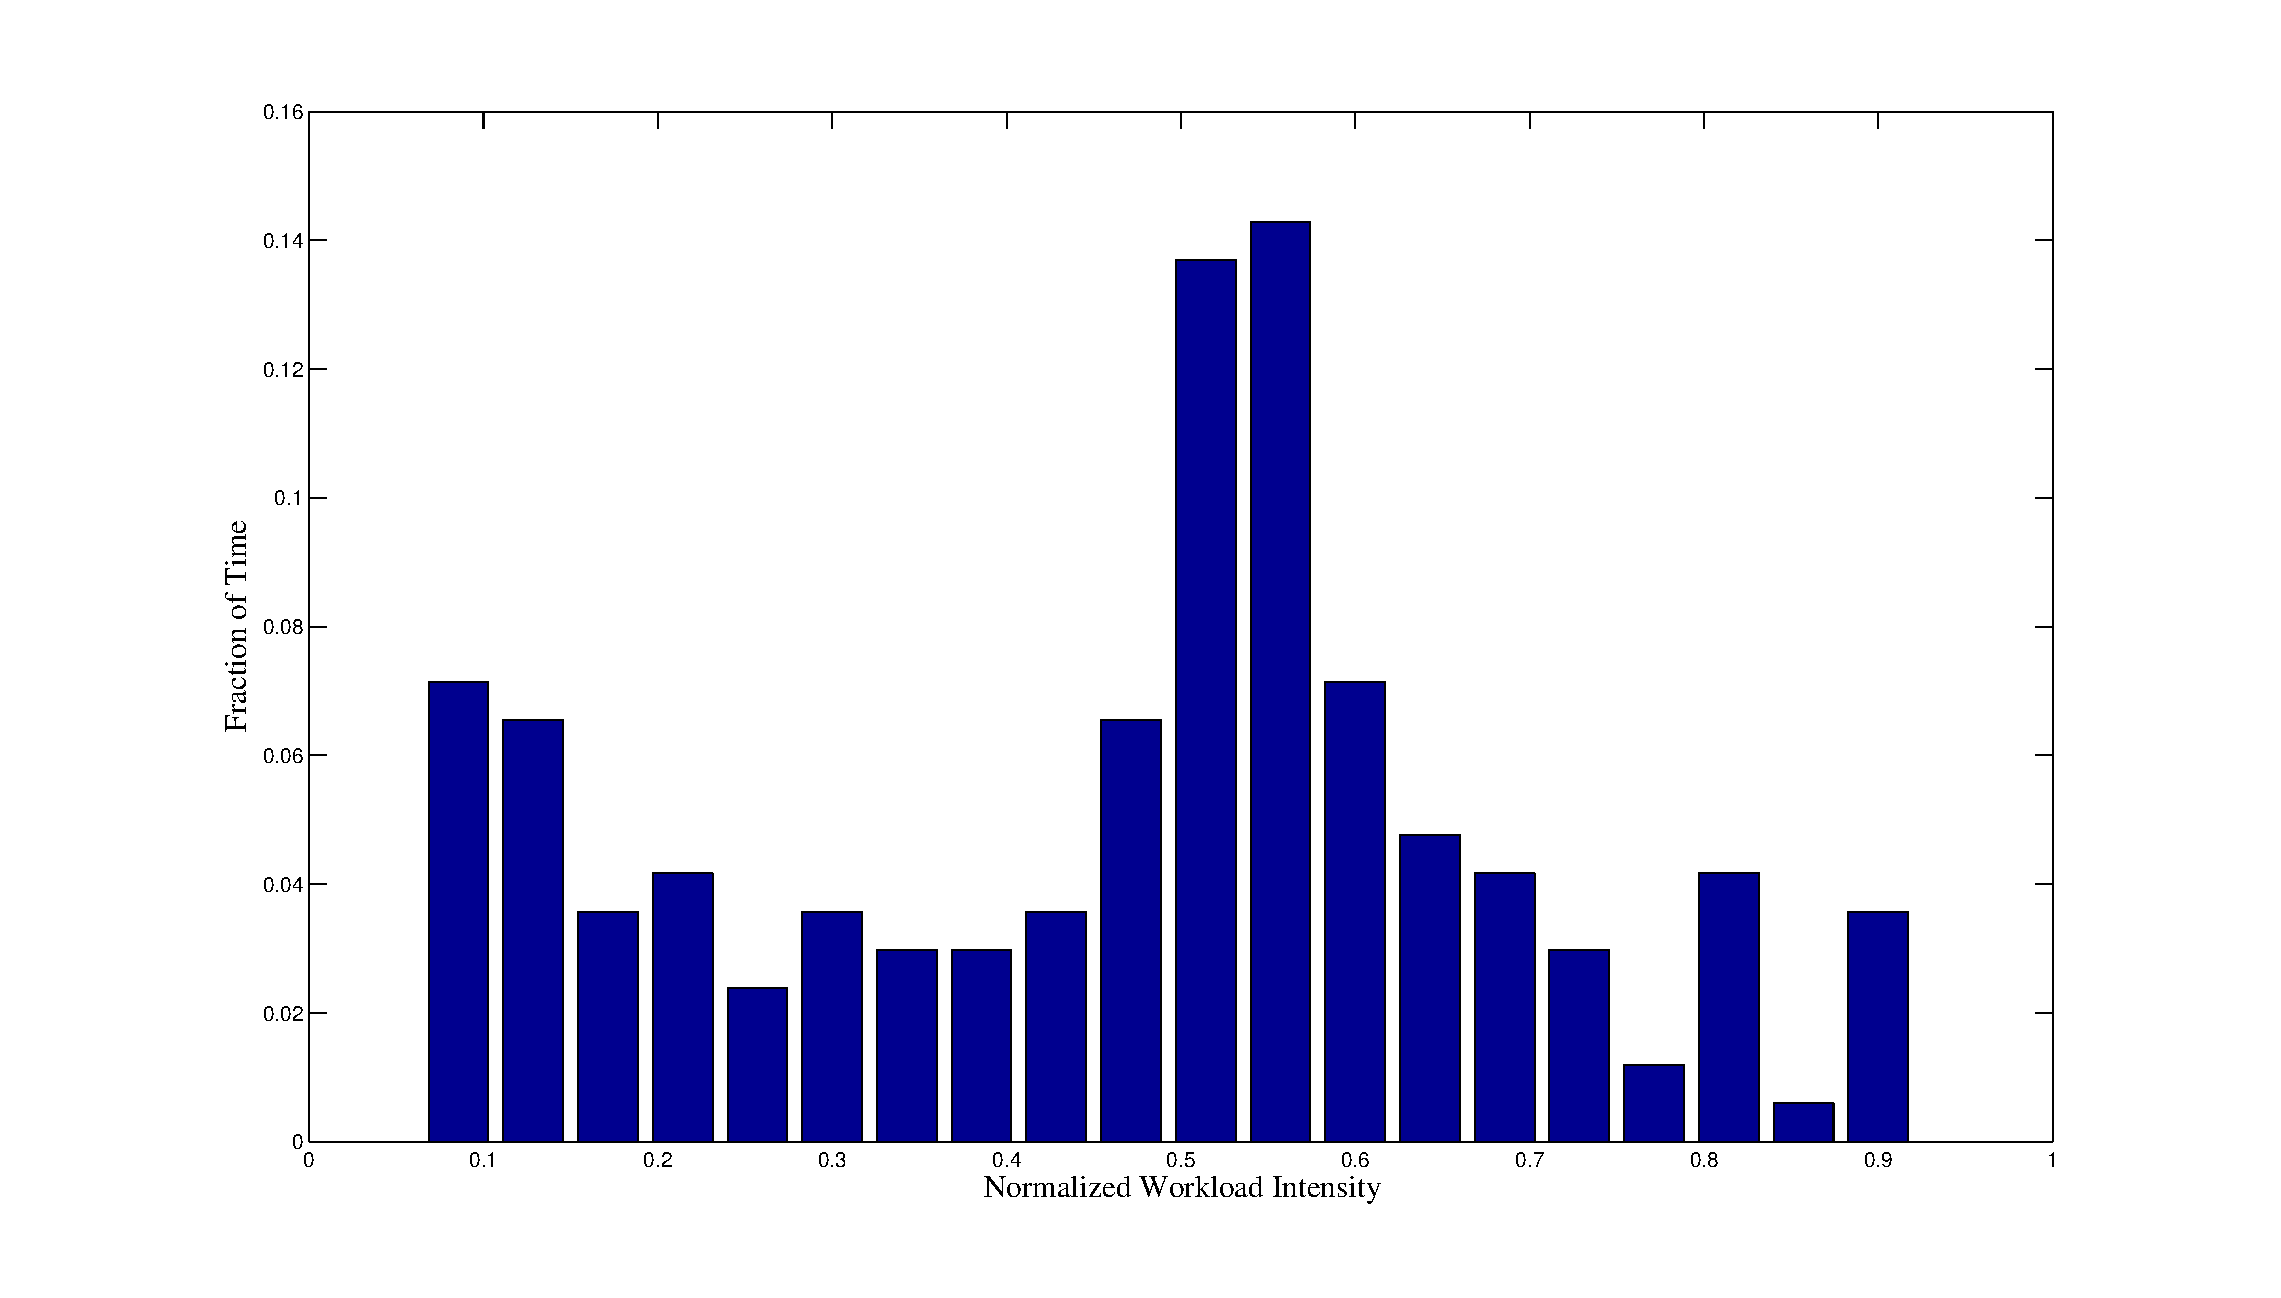
\includegraphics[width=\linewidth]{pics/workloadhist-new.eps}
    \caption{Workload intensity histogram}
    \label{fig:workloadhist}
  \end{minipage}
\end{figure}

\subsection{Electricity prices}
\label{subsec:prices} We selected $33$ different regions in the USA for which hourly electricity prices are available online. These regions belong to the following Independent System Operators (ISOs): NYISO, CAISO, MISO, ISO-NE and PJM. %To ease reproducibility of our results, the names for these locations as used in the online datasets are listed in Table~\ref{tab:locations}. 
We used the day-ahead prices for these locations, i.e., the electricity price negotiated for the same hour on the following day. In all the experiments for this thesis, we considered an operator with data centers at all 33 locations in our dataset. 

%\begin{table}
%\begin{center}
%\scalebox{0.7}
%{
%\begin{tabular}{|c|c|c|c|c|c|c|c|c|c|c|c|}
%\hline S. No. & Source & S. No. & Source & S. No. & Source & S. No. & Source & S. No. & Source & S. No. & Source \\
%\hline 1 & CAPITL & 7 & LONGIL & 13 & OH & 19 & MISO & 25 & WCMass & 31 & SEMass \\
%\hline 2 & CENTRL & 8 & MHKVL & 14 & PJM1 & 20 & Illinois & 26 & Boston & 32 & Vermont\\
%\hline 3 & DUNWOOD & 9 & MILLWD & 15 & WEST & 21 & Cinergy & 27 & CT & 33 & PJM2\\
%\cline{1-10} 4 & GENESE & 10 & NYC & 16 & PGAE & 22 & Michigan & 28 & Maine & \ & \ \\
%\cline{1-10} 5 & HQ & 11 & NORTH & 17 & SCE & 23 & Minnesota & 29 & NH  & \ & \ \\
%\cline{1-10} 6 & HUDVL & 12 & NPX & 18 & SDGE & 24 & First Energy & 30 & Rhode & \ & \ \\
%\hline
%\end{tabular}
%}
%\caption{Sources of electricity prices used in our work}
%\label{tab:locations}
%\end{center}
%\end{table}

%\begin{table}
%\begin{center}
%\begin{tabular}{ll}
%\hline Algorithm & Remarks \\
%\hline LI & Local optimal with idling \\
%LD & Local optimal with deactivation \\
%LS & Local optimal with selection \\
%LO & Local optimal without transition costs \\
%RED-BL & The global optimal solution for the planning window\\
%UNIFORM & Distribute workload equally over all data centers in all intervals \\
%%STATIC\_MIN & A single site data center operator \\ 
%\hline
%\end{tabular}
%\caption{Algorithms compared in our work}
%\label{tab:algos}
%\end{center}
%\end{table}

\subsection{Algorithms for Workload Distribution/Relocation}
\label{subsec:metrics} The workload relocation problem has the following dimensions based on which different algorithms may be formulated. 

\begin{itemize}
\item For a given interval, the strategy for distribution of workload amongst data centers.
\item For a given interval, the strategy for the state (on/off) of elastic load at a data center which has not been assigned any workload. In such cases, there is a trade-off between keeping the elastic load on (and incurring idling costs) and deactivating it (while incurring deactivation overhead and possibly activation overhead if it needs to be brought back online later in the planning window).
\item Over the planning window, does the algorithm report transition costs in the total electricity cost?
\end{itemize}

In this thesis, we report comparative results for six workload placement algorithms.%, listed in Table~\ref{tab:algos}. 
 The following list describes and differentiates these algorithms. The same comparison is also presented in tabular form in Table~\ref{tab:algosmatrix}.

\begin{itemize}
\item \textbf{RED-BL:} This is our proposed algorithm that determines the global optimal cost of electricity over a planning window while considering and reporting the transition costs. The choice of workload distribution as well as the state of elastic resources with no workload is governed by the optimal solution as determined by the CPLEX solver.
\item \textbf{Heuristic:} This is the heuristic algorithm that we proposed in Section~\ref{subsec:complexityheur}.
\item \textbf{UNIFORM:} This algorithm represents the choice of those operators that find an even loading of their data centers desirable. This algorithm does not deactivate elastic loads and hence does not incur transition costs.
\item \textbf{Greedy algorithms:} The originally proposed algorithm in~\cite{qureshi2009cutting} distributes workload to data centers such that, for each interval in the planning window, it makes a greedy assignment (in terms of current electricity price) of workload to data centers. Furthermore, this original algorithm keeps the elastic load at all data centers active in all intervals, incurring significant idling costs and hence is naturally disadvantaged against RED-BL. To have a fair comparison with the greedy workload distribution strategy, we use several variants of the original algorithm as well.
\begin{itemize}
\item \textbf{Local optimal with Idling (LI):} This is the originally proposed algorithm from~\cite{qureshi2009cutting}. It does not deactivate elastic load.
\item \textbf{Local optimal withOut transition costs (LO):} This variant of LI was proposed in~\cite{qureshi2009cutting}. It deactivates un-needed elastic load while ignoring the transition costs. This algorithm does not report transition costs in the total electricity cost of it's proposed workload mapping for the planning window. This algorithm is very useful because it defines the lower bound on electricity cost that any algorithm can ever achieve.
\item \textbf{Local optimal with Deactivation (LD):} This algorithm is similar to LO in all respects except that it also reports the activation/deactivation costs as part of the total cost of it's proposed solution. Unlike LO, it's results are practically relevant. It's total cost is less than (for all practical cases) LI, which makes it somewhat competitive to RED-BL.
\item \textbf{Local optimal with Selection (LS):} In cases where transition costs are high compared to idling costs it would be better to keep the elastic resources at a data center active and incur idling costs if it will be needed again after the lapse of a small number of intervals. LS is a variant of LD that is empowered with the ability to \textit{select} whether to deactivate unneeded elastic load at a data center or keep it idling. The cost of LS is never greater than that of LD.
\end{itemize}
\end{itemize}

\begin{table}
\begin{center}
\begin{tabular}{|c|c|}
\hline \multicolumn{2}{ |c| } {\bf{Workload mapping strategy}}\\
\hline LI, LD, LS, LO & Greedy \\
\hline RED-BL & Based on global optimal solution \\
\hline UNIFORM & Workload equally divided amongst all data centers \\
\hline \multicolumn{2}{|c|}\ \\
\multicolumn{2}{ |c| } {\bf{State of a data center in an interval when it has no workload}}\\
\hline LI & Active and idling \\
\hline LD, LO & Inactive \\
\hline LS & Either inactive or idling, whichever is cheaper \\
\hline RED-BL & Based on global optimal solution \\
\hline UNIFORM & Active \\
\hline \multicolumn{2}{|c|}\ \\
\multicolumn{2}{|c|}{\bf{Is transition cost reported in the total electricity cost reported?}}\\
\hline LI & N/A \\
\hline LD, LS & Yes \\
\hline LO & No \\
\hline RED-BL & Yes \\
\hline UNIFORM & N/A \\
\hline
\end{tabular}
\caption{A comparison of the algorithms studied in this thesis}
\label{tab:algosmatrix}
\end{center}
\end{table}


\section{Results}
 To evaluate the utility of workload relocation for electricity cost minimization, we
formulated seven different scenarios. For each scenario, we ran
seven experiments (one for each day's workload in our dataset) and report the average of the total electricity cost for each algorithm. Each experiment determines an operational plan for a planning window consisting of $24$ consecutive intervals, each with a duration of one-hour.

\begin{figure}
\centering
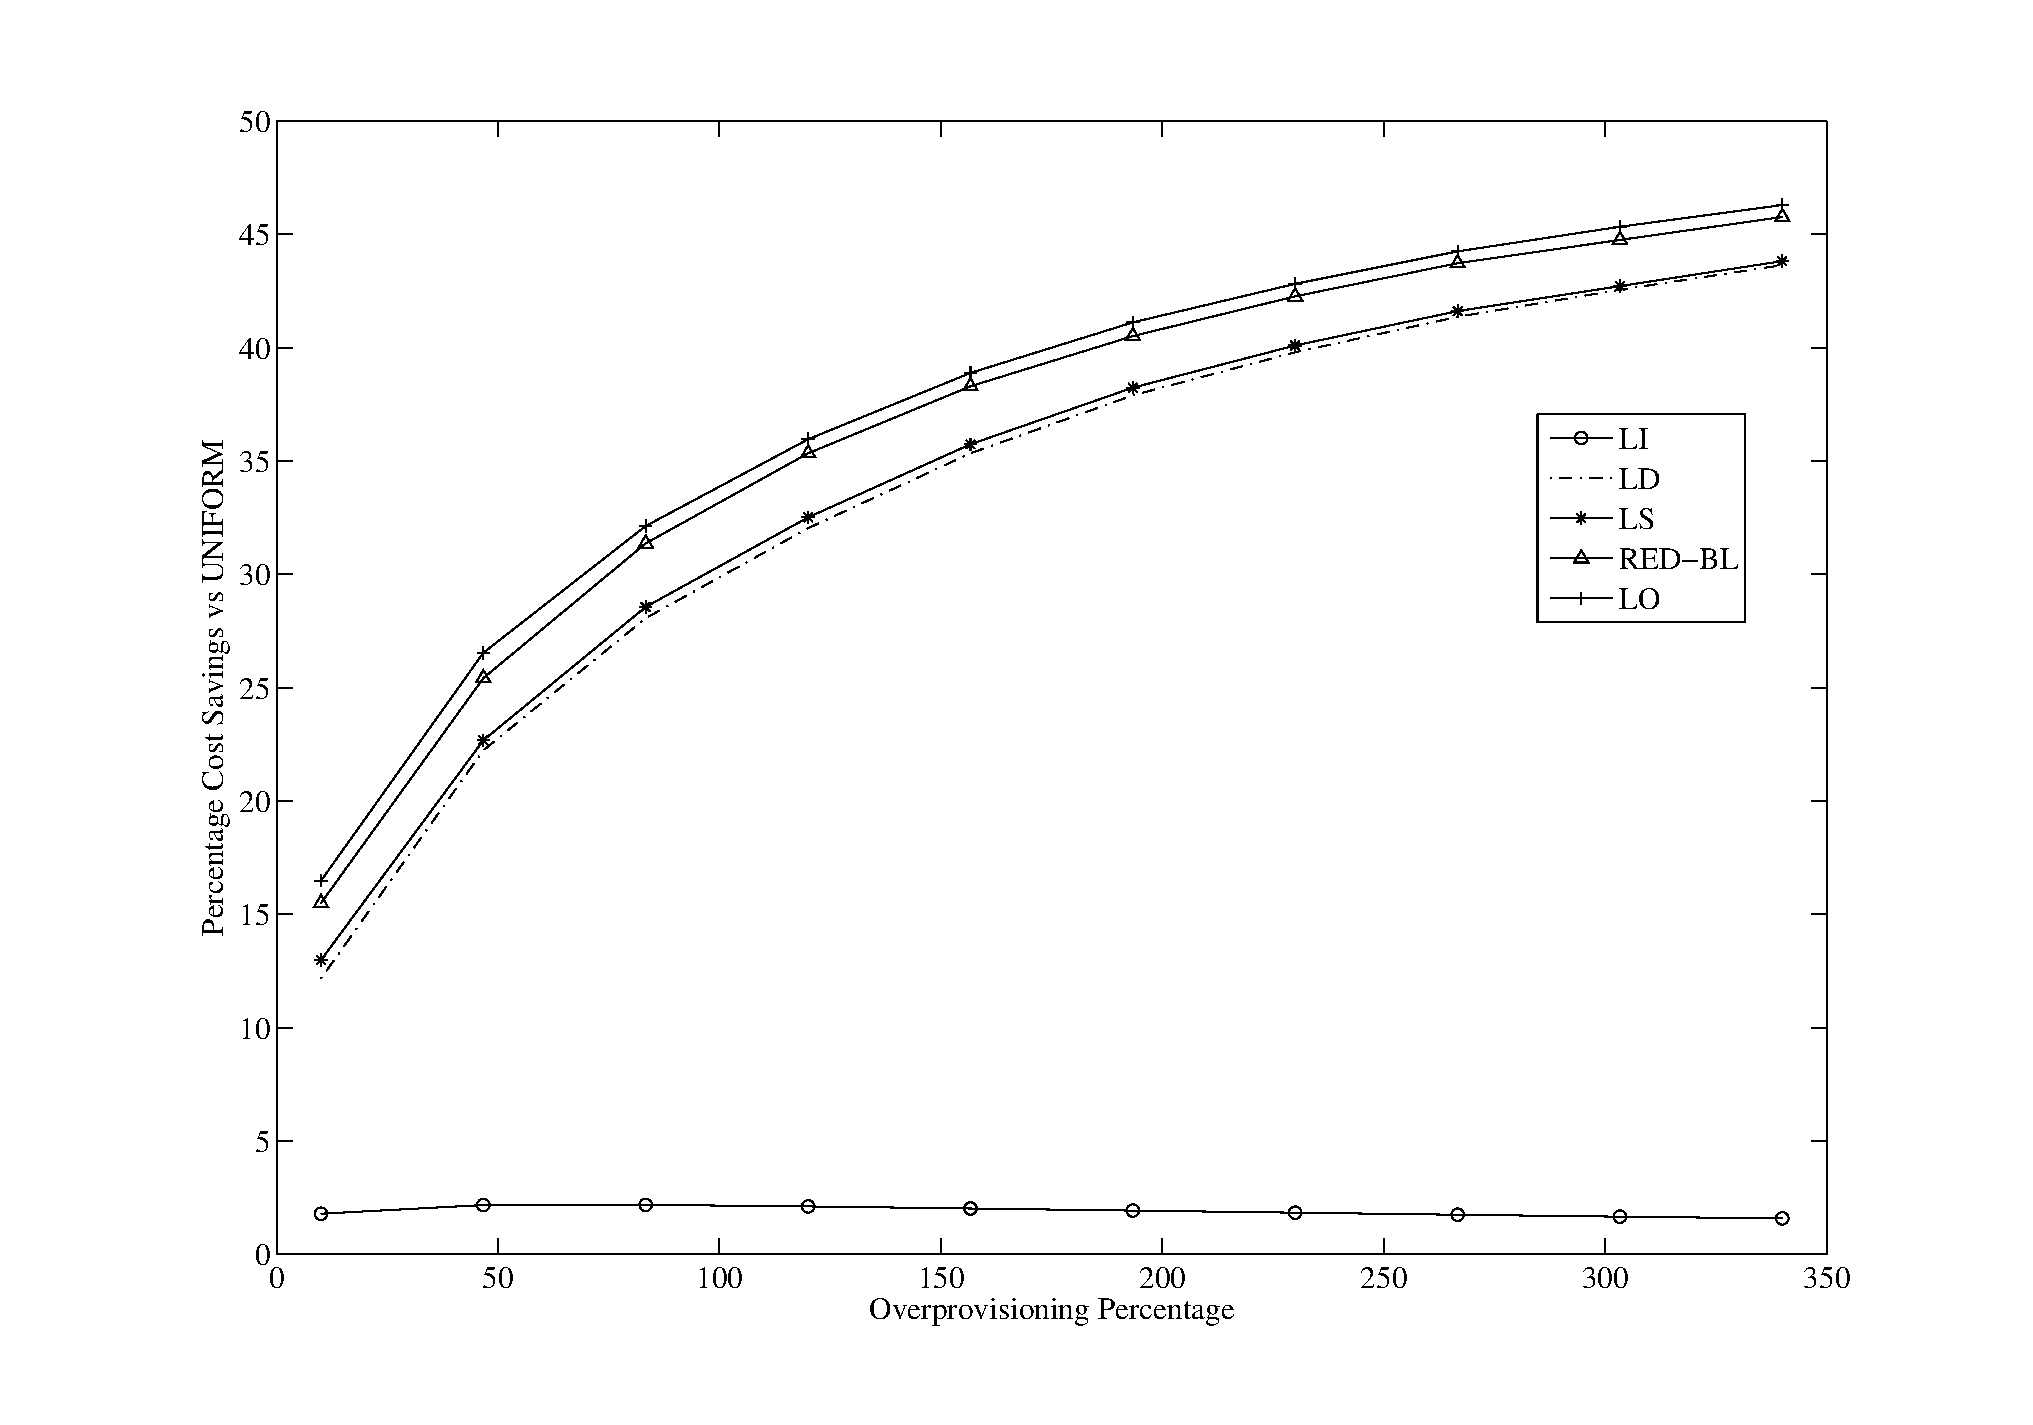
\includegraphics[width=0.7\textwidth]{pics/s1vseqr.eps}
    \caption{Percentage savings with over-provisioning}
    \label{fig:s1r}
\end{figure}

\subsection{Sensitivity of electricity cost savings to extent of over-provisioning}In this scenario, we investigate the relationship of the amount of data center capacity over-provisioning with the electricity cost savings. As we increase the amount of over-provisioning, each individual data center's capacity would increase enabling more and more workload to be mapped to data centers at locations with cheaper electricity price.

With data centers at all
    $33$ locations in our dataset, we varied $c_i$ between $0.03$ and
    $0.12$ (in increments of $0.01$). This covers a variety of operators whose workload capacity ranges from just over expected peak workload to
almost $300\%$ over-provisioning.

We computed the total electricity cost for all algorithms while setting $f=\sigma=\delta=0.65$. The percentage savings in total electricity cost by various algorithms compared to UNIFORM are plotted against the data center capacity over-provisioning in Figure~\ref{fig:s1r}. We found that for the wide range of capacity over-provisioning that we considered, LI is able to do only slightly better than the naive UNIFORM algorithm (about 2\%). This is due to the significant idling costs incurred by LI under the experiment's conditions. For this reason, we have omitted LI from this plot.

The most competitive practical variants of LI, i.e., LS was 10.35\% off from the ideal lower bound (LO). Meanwhile, RED-BL solution is quite close the ideal lower bound (LO). The reason for greater savings with RED-BL compared to the greedy solutions (LS and LD) is that, the transition costs being significant, the former does fewer state transitions. In several intervals, RED-BL chooses data centers with relatively higher electricity price than the greedy solutions, but makes up for the higher computational cost by a reduction in the transition costs incurred.

\subsection{Sensitivity of electricity cost savings to magnitude of transition costs}
As the magnitude of transition costs relative to the state cost for an interval grows beyond a certain point, the benefits of deactivating elastic load at data centers would diminish. Accordingly, the electricity cost savings achievable by the workload relocation schemes would drop with increase in transition costs. In this scenario, we determine the percentage savings in total
    electricity cost for each algorithm, except
    STATIC\_MIN\footnote{STATIC\_MIN uses a static workload mapping so it is insensitive to variations in transition costs}, compared to UNIFORM, while varying the activation/deactivation overhead
    between $0$ and $1$, in increments of
    $0.1$. The lower bound on $\sigma$ (and $\delta$)
    implies the ideal condition of no transition overheads.
    We set the upper bound to $1$ so that the
    transition costs equal the cost of operating a data
    center at full load for an interval. A transition cost
    higher than this does not make sense as a workload relocation scheme would be better off keeping the elastic load at unloaded data centers idle. In this scenario,
    we kept $f=0.65$.

LI does not (de)activate unneeded elastic load and thus it's electricity cost is independent of the magnitude of transition costs. We observed taht it offered a saving of merely 1.74\% compared to UNIFORM. Figure~\ref{fig:s3r} shows the electricity cost savings for the other algorithms compared to UNIFORM. The LS and LD adaptations of the LI algorithm offer savings that scale almost linearly to the magnitude of transition costs. Both LS and LD also bring an average reduction in the elastic load's electricity cost sby a factor of $4$, compared to that of LI. RED-BL not only scales better than LS and LD but also achieves electricity cost saving that is fairly close (only $3\%$ higher, on average) than the ideal lower bound as reported by LO.


\begin{figure}[htbp]
  %\begin{minipage}[b]{0.5\linewidth}
    \centering
    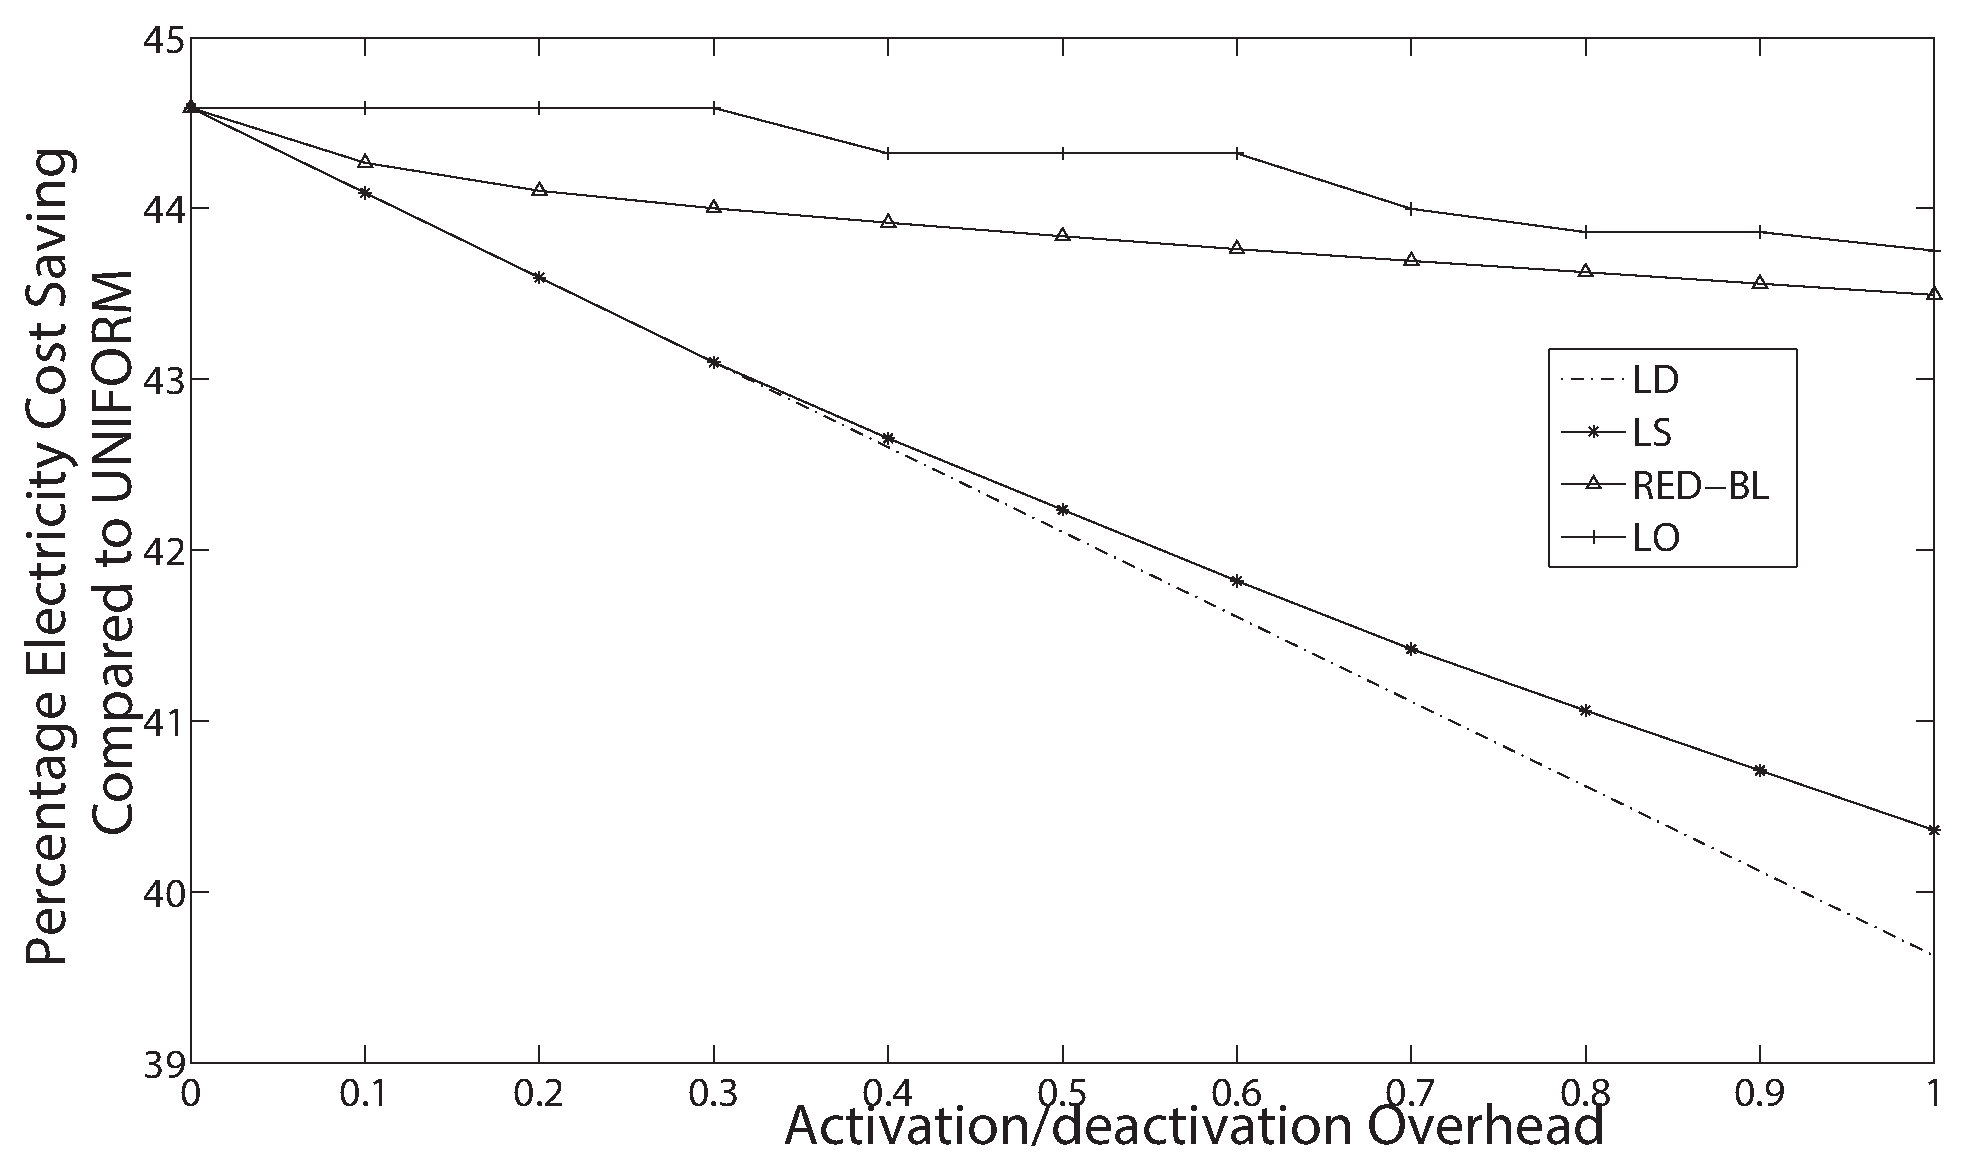
\includegraphics[width=0.7\linewidth]{pics/s3r.eps}
    \caption{Total cost vs transition overhead}
    \label{fig:s3r}
  %\end{minipage}
  %\hspace{0.5cm}
%  \begin{minipage}[b]{0.5\linewidth}
%    \centering
%    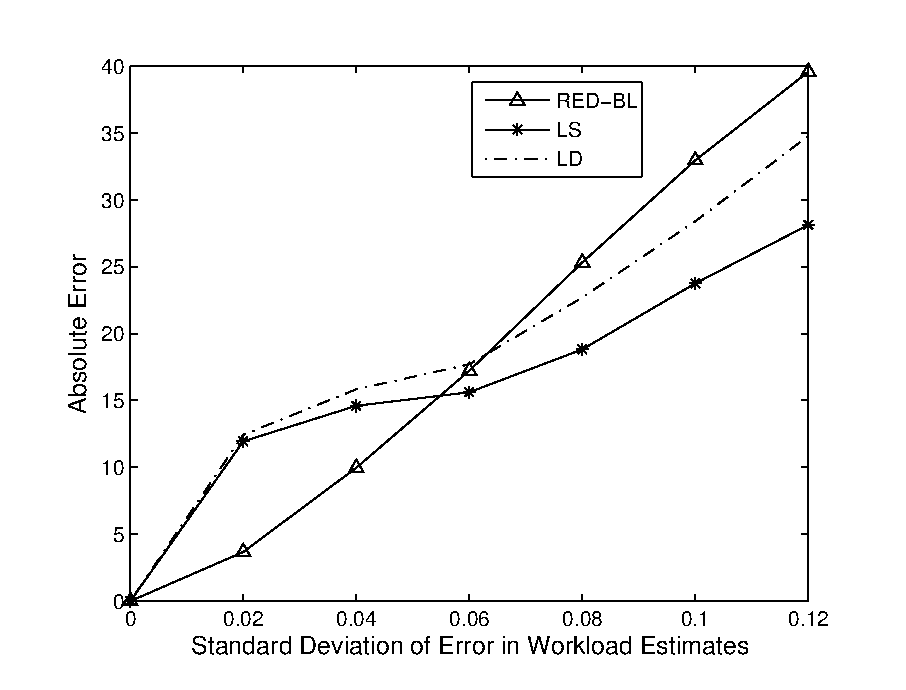
\includegraphics[width=1\linewidth]{pics/s4.eps}
%    \caption{Cost estimation error due to workload estimation error}
%    \label{fig:s4r}
%  \end{minipage}
\end{figure}

\subsection{Sensitivity of electricity cost savings to resource pruning granularity}
In this scenario, we investigate the potential benefits of deactivating the elastic load in a data centers in equal sized chunks instead of an all or nothing approach. The size of the portion of the elastic load in a data center that may be independently (de)activated may be deployment-dependent or operator-dependent. Possible choices of granularity may be a rack, a pod or one half of the elastic load etc. This granular deactivation can also be seen as throttling the equipment in a data center using facilities like processor frequency scaling. 

Granular (de)activation is expected to bring additional power savings. For instance, if the elastic load in a data center is operating at 10\% of it's capacity, then the remaining 90\% of the load is still consuming significant idling power. If we had the ability to power down half of the elastic load at a data center, we could cut idling energy cost significantly. 

The optimization problem formulation with $l$ granular (de)activation levels is given by:
 
\begin{align}
\text{minimize } \sum_{j=1}^{n} \sum_{i=1}^{m} c_i e_i^j\left(p_i^j \lambda\left(\frac{f}{l}+\left(1-f\right)\frac{x_i^j}{c_i}\right) + \frac{b_i^j \sigma}{l} + \frac{s_i^j \delta}{l}\right)\notag
\end{align}
subject to:
\begin{align}
x_i^j \le c_i \hspace{6 pt} \forall i, \forall j \label{eq:gcapcon}\\
\sum_{i = 1}^{m} x_i^j = w^j \hspace{6 pt} \forall j \label{eq:gworkcon}\\
p_i^j, b_i^j, s_i^j \in \{0,1,...,l\} \hspace{6 pt} \forall i, \forall j \label{eq:ginteger1}\\
p_i^j \ge x_i^j*l/c_i \hspace{6 pt} \forall i, \forall j \label{eq:gp1}\\
b_i^j \ge p_i^j - p_i^{j-1} \hspace{6 pt} \forall i, 2 \le j \le n \label{eq:gbcon}\\
%\end{align}
%\begin{align}
s_i^j \ge p_i^{j-1} - p_i^j \hspace{6 pt} \forall i, 2 \le j \le n \label{eq:gscon}\\
b_i^0 = p_i^0, s_i^0 = 0 \hspace{6 pt} \forall i \label{eq:gbcon1}
\end{align}

There are three primary differences from the vanilla RED-BL formulation. The first difference is in the objective function, where the idling, bootup and shutdown costs depend on the number of granular units involved in the idling, bootup or shutdown process respectively. Since the computational cost component of power consumption only depends on the workload and is independent of the data center capacity, it is independent of the number of granular units being used at a data center during a given interval. The second difference is in the domain of $p_i^j$, $b_i^j$ and $s_i^j$ (see constraint~\ref{eq:ginteger1}). The third difference is in the constraint~\ref{eq:gp1}, which ensures that $p_i^j$ takes on an appropriate value from $0,1,...,l$.

\begin{figure}
    \centering
    \includegraphics[width=0.7\textwidth]{pics/s6.eps}
\caption{Cost saving vs (de)activation granularity}
\label{fig:granular-deactivation}
\end{figure}

In the current evaluation scenario, we explore how the RED-BL electricity cost savings scale with change in size of the unit of independent (de)activation. In Figure~\ref{fig:granular-deactivation}, we have plotted the percentage savings in electricity cost vs the granularity of data center's elastic load (de)activation. The savings are computed against the scenario where only the entire elastic load in the data center may be (de)activated as a whole. This baseline corresponds to a value of $l$ equal to one. Accordingly, in Figure~\ref{fig:granular-deactivation} we see no savings for that value of $l$. We also see that the ability to independently (de)activate half of a data center's elastic load provides around $2.5\%$ additional such savings on top of what the vanilla RED-BL can achieve. The electricity cost savings grow almost linearly when going to more granular size of independent (de)activation.

\subsection{Sliding window re-optimization}
With the exception of scenario 3, all of our simulation scenarios have been driven by error-free workload traces. The underpinning assumption to the corresponding results, therefore, is the availability of accurate workload estimates. We opine that this is not such a bad assumption given that the cumulative workload on the granularity of an hour changes slowly from one hour to the next and from one hour on a day to the same hour the next day. However, workload forecasting will have some error, however small it may be. 

In order to accommodate workload mis-estimation, we propose a sliding window-based algorithm that is somewhat similar to receding horizon control~\cite{rhc}. The algorithm is so called because it performs workload forecasts for a planning window and later slides the window by a constant offset before making another workload forecast, this time for intervals currently in the planning window. 

Our approach compensates for workload estimation errors on two (often) different time-scales. At an (often) longer timescale, the workload for the next $n$ intervals is forecast and a RED-BL plan is generated. This forecasting is repeated every $\gamma$ intervals, the \textit{window slide interval} parameter. The motivation is that at interval number 1, the workload forecast for interval number $gamma+k$ is expected to contain a greater amount of error than if the forecast for the same interval is done at interval $\gamma$, due to availability of more historical workload data at the later interval. This step of repeated forecasting and subsequent generation of a RED-BL plan is called \textit{global trajectory correction}. The basic idea behind this approach is that lowering of workload estimation error should bring the planned state trajectory closer to the optimal state trajectory (the one that results from perfect workload estimates). 

On a relatively shorter timescale, in each interval, our algorithm locally corrects for forecasting errors. The planned state for an interval may be \textit{infeasible} in the sense that it may be based on an under-estimation of workload and we might not have sufficient active data center capacity for the actual workload. Also, in case of over-estimation of workload, the originally planned state may be \textit{locally sub-optimal} as some data center resources would unnecessarily consume idling costs. This step that corrects for locally infeasible or sub-optimal states, considers only a single interval and, hence, is called \textit{local trajectory correction}. Upon entering an infeasible or locally sub-optimal planned state, we perform a local correction by finding a new state for the current interval. As shown in Figure~\ref{fig:traj-corr}, we start at the initial state $S_0$ and are scheduled to transition to state $\hat{S}_1$ at interval $1$. However, at interval $1$, we know the actual workload received and might discover that the planned state is locally infeasible or sub-optimal. To accommodate this, we transition to a locally better state $S_1$. At the end of interval $1$, we are scheduled to transition to state $\hat{S}_2$, and the process repeats. Since we only have accurate information about the workload for the present interval, the revision of the next state is always deferred to the next local trajectory correction step.

The local trajectory correction for interval $j$ is an optimization problem that attempts to minimize the electricity cost of the corrected state $S_j$ and the cost of transition between the planned state $\hat{S}_j$ and the corrected state. The mixed integer linear programming formulation for the local trajectory correction step for interval $j$ is as follows:
    
\begin{align}
\text{minimize } \sum_{i=1}^{m} c_i e_i^j\left(p_i^j \lambda\left(f+\left(1-f\right)\frac{x_i^j}{c_i}\right) + \left(b_i^j+\hat{b}_i^j\right) \sigma + \left(s_i^j+\hat{s}_i^j\right) \delta\right)
\end{align}
subject to:
\begin{align}
x_i^j \le c_i \hspace{6 pt} \forall i \label{eq:lcapcon}\\
\sum_{i = 1}^{m} x_i^j = w^j \hspace{6 pt} \label{eq:lworkcon}\\
p_i^j, b_i^j, s_i^j \in \{0,1\} \hspace{6 pt} \forall i \label{eq:linteger1}\\
p_i^j \ge x_i^j \hspace{6 pt} \forall i \label{eq:lp1}\\
b_i^j \ge p_i^j - \hat{p}_i^j \hspace{6 pt} \forall i \label{eq:lbcon}\\
s_i^j \ge \hat{p}_i^j - p_i^j \hspace{6 pt} \forall i \label{eq:lscon}\\
\hat{b}_i^j \ge \hat{p}_i^j - p_i^{j-1} \hspace{6 pt} \forall i \label{eq:lbcon1} \\
%\end{align}
%\begin{align}
\hat{s}_i^j \ge p_i^{j-1} - \hat{p}_i^j \hspace{6 pt} \forall i \label{eq:lscon1}
\end{align}

\begin{figure}
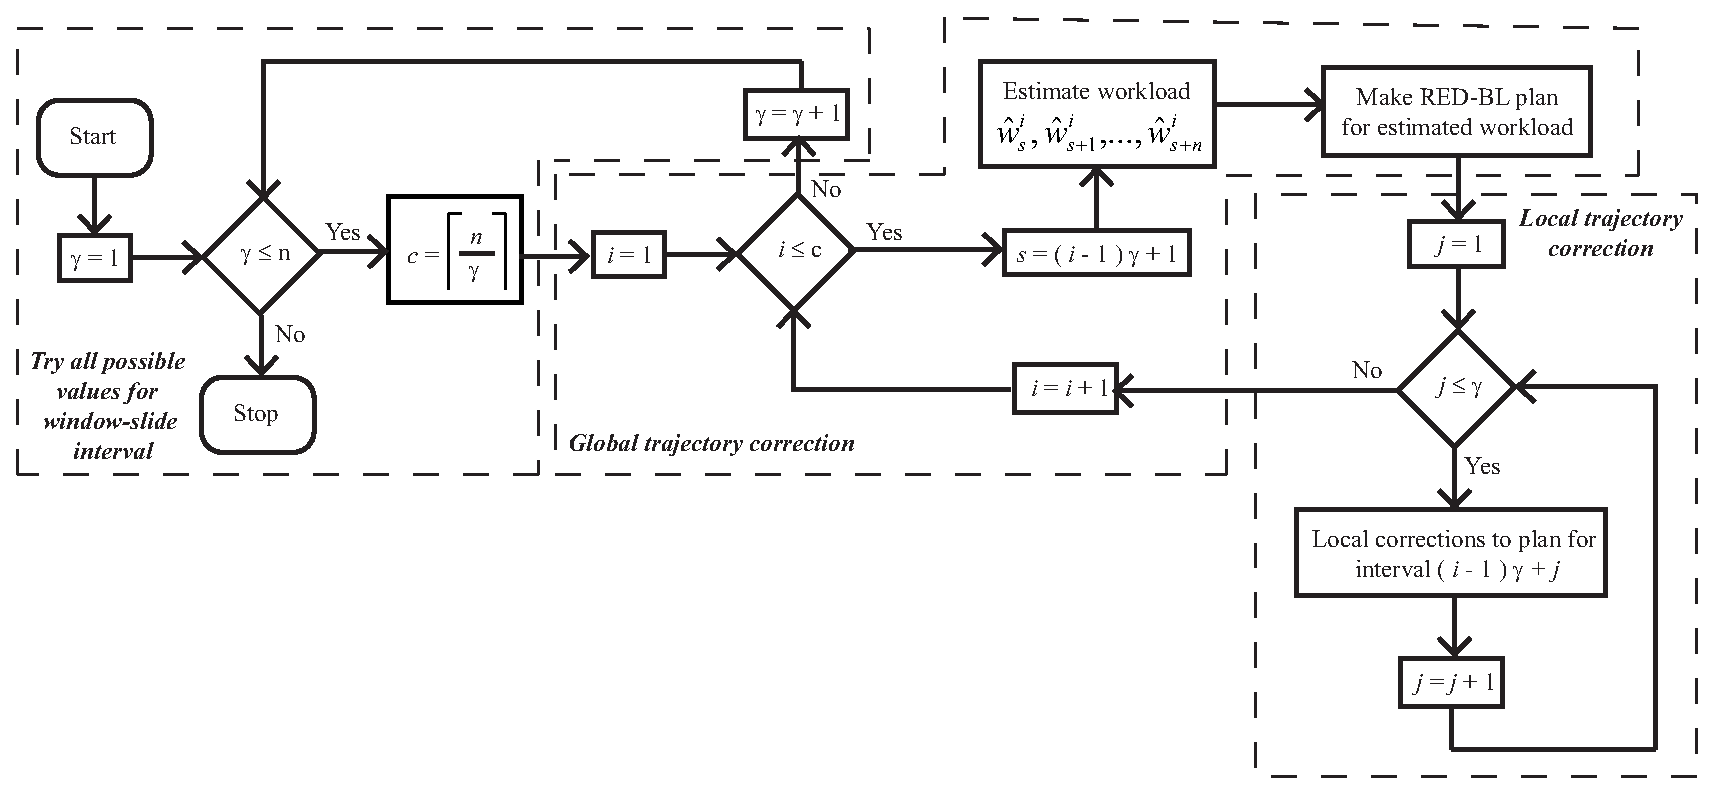
\includegraphics[width=1\linewidth]{pics/flowchart3.eps}
\caption{Flow of sliding window experiments}
\label{fig:flowchart}
\end{figure}

\begin{figure}[htbp]
  \begin{minipage}{0.45\textwidth}
    \centering
    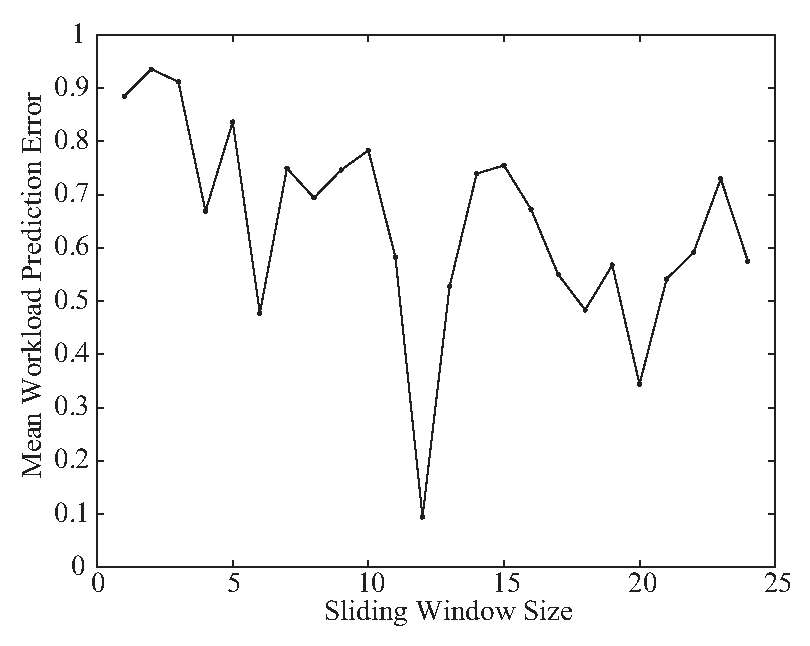
\includegraphics[width=0.8\textwidth]{pics/workload-pred-error-mean.eps}
    \caption{Mean absolute workload prediction error vs sliding window size}
    \label{fig:workload-pred-error-mean}
  \end{minipage}
  %\hspace{0.5cm}
  \begin{minipage}{0.45\textwidth}
    \centering         
    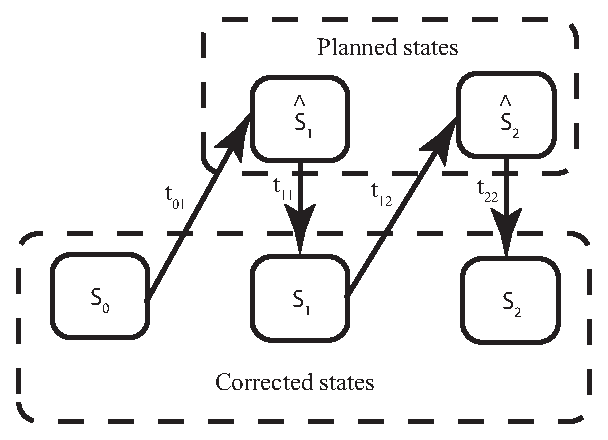
\includegraphics[width=0.8\textwidth]{pics/traj-corr2.eps}
    \caption{Local trajectory correction technique for three consecutive intervals}
    \label{fig:traj-corr}
    \end{minipage}
\end{figure}

\begin{figure}
\centering
\includegraphics[width=0.7\linewidth]{pics/workload-pred-error-2.eps}
    \caption{Distribution of workload prediction error for sliding window size of 12 hours}
    \label{fig:workload-pred-error-dist}
    \end{figure}
    
    Given that the planning window size is $n$ intervals, the possible values for $\gamma$ are $1, 2, .., \gamma$. We experimented with all possible values for $\gamma$. Figure~\ref{fig:flowchart} shows the flow of our experiments. We first pick a value for the window sliding interval and estimate the workload for the next $n$-intervals and then invoke RED-BL. As an example, consider $\gamma=2$. We start by forecasting the workload for the first $n$-intervals, denoted by $\hat{W}_1^2 = [\hat{w}_{1,1}^2, \hat{w}_{2,1}^2, ..., \hat{w}_{n,1}^2]$. Here, $\hat{w}_{j,1}^2$, for instance, represents the workload forecast for interval $j$ during the first forecasting operation while the value of $\gamma$ is 2. For workload forecasting, we trained an ARMA(4, 4)~\cite{arma} model on a day's workload. Using $\hat{W}^2_1$ as the expected workload vector, we propose a RED-BL deployment plan for the first $n$-intervals. After the lapse of $\gamma$ intervals, i.e., at the start of the third interval (for $\gamma$ = 2), we forecast the workload for the next $n$ intervals, leveraging the additional information about the actual workload for the first two intervals which was not available in the first forecast step at $t=0$. This forecast is denoted by $\hat{W}_2^2 = [\hat{w}_{3,2}^2, \hat{w}_{4,2}^2, ..., \hat{w}_{n+2,2}^2]$. Then, we compute the RED-BL deployment plan for intervals $3, 4,..., n+2$ as the global trajectory correction step. Since the window sliding interval size is $\gamma$ and the number of intervals in our experiments is $n$, the number of times the window must slide, for a given value of $\gamma$ is $\lceil n/\gamma \rceil$. For $\gamma$ = 1, our scheme reduces to something resembling receding horizon control.
    

Having trained the model on the first day's data, we ran experiments for the last six days' workload in our dataset. We computed the average error of the daily electricity cost reported by these experiments compared to the total daily electricity cost for the same period with perfect workload estimates. The size of the planning window was set to 24 hours. 

The first set of results in this scenario is the percentage workload estimation error for various sliding window sizes. We see in Figure~\ref{fig:workload-pred-error-mean} that the mean absolute percentage prediction error is less than $1\%$. The minimum mean error is for a sliding window size of $12$ hours. For this sliding window size, the distribution of percentage workload estimation error is plotted in Figure~\ref{fig:workload-pred-error-dist}. Most of the workload estimates are quite close to error-free, while a few estimates are as much as 24$\%$ off. This low average error for $\gamma$ = 12 is expected due the nature of daily variations in the cumulative workload.

The difference of the electricity cost resulting from the use of the sliding window trajectory correction approach compared to the optimal solution with perfect workload knowledge is plotted in Figure~\ref{fig:s5r}. We see that the electricity cost achievable with RED-BL in a sliding window fashion is within 5-7$\%$ of the optimal cost achievable with perfect workload estimates. 

\begin{figure}[htbp]
    \centering
    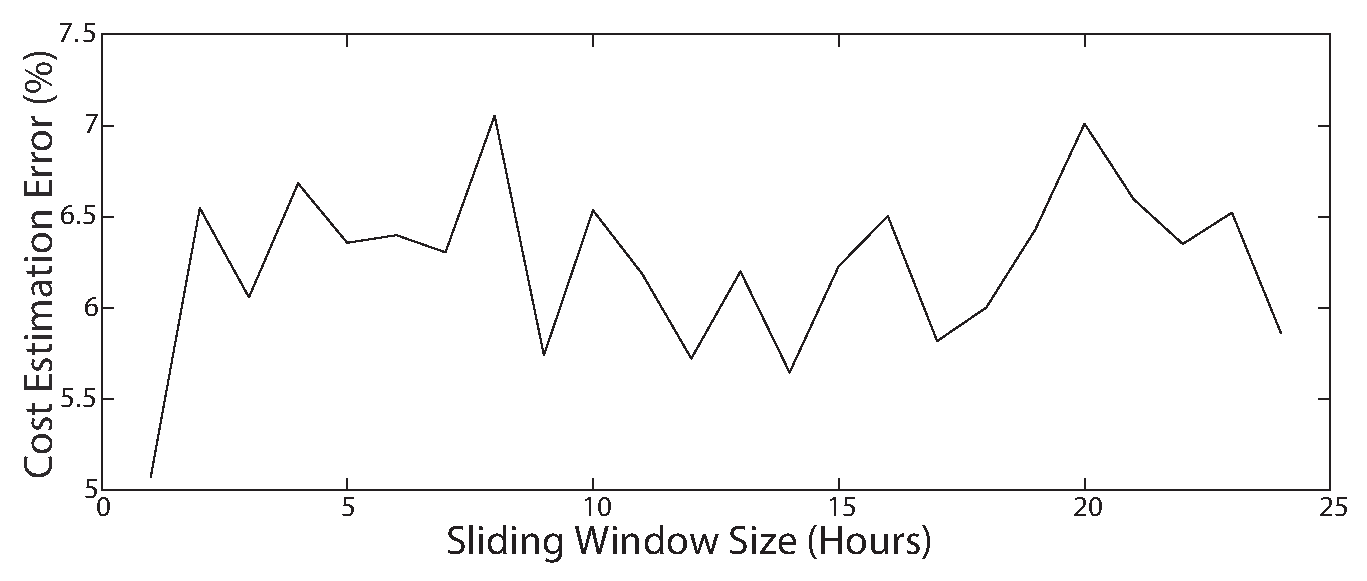
\includegraphics[width=0.8\textwidth]{pics/sw-cost-error-2.eps}
\caption{Percentage error of sliding window forecasts compared to global optimal with error-free workload}
\label{fig:s5r}
\end{figure}



\subsection{Sensitivity of electricity cost savings to the server idle-peak power ratio}
Chip manufacturers and computer vendors are striving to improve server energy propotional/efficient. It would be interesting to see how the electricity cost savings for RED-BL would improve as the server's idle to peak power ratio ($f$) drops. To this end, we conducted a set of experiments in which we kept all other parameters fixed while varying $f$ from 0 to 1.  Note that $f$=0 means that the servers are completely energy proportional, whereas $f$=1 means that the server power consumption is totally inelastic.

Figure~\ref{fig:fvar1} shows the variation of electricity cost savings as the value of $f$ is varied while the $b$/$s$ parameteres are kept at a low value of 0.01. In this setting, we wish to investigate if server energy proportionality improvement really matters if the bootup/shutdown costs were really low. Figure~\ref{fig:fvar1} shows that for an increase from $f$=0 to $f$=1, the global optimal solution over the planning window only spans an increase in average total electricity cost of 8.34\%. Also, a drop from the typical $f$=0.6 all the way to $f$=0 results in a 4.88\% drop in total electricity cost. It is noticeable that the bootup/shutdown overheads are really small and the idling fraction of electricity costs increases almost linearly with the value of $f$.
 
\begin{figure}
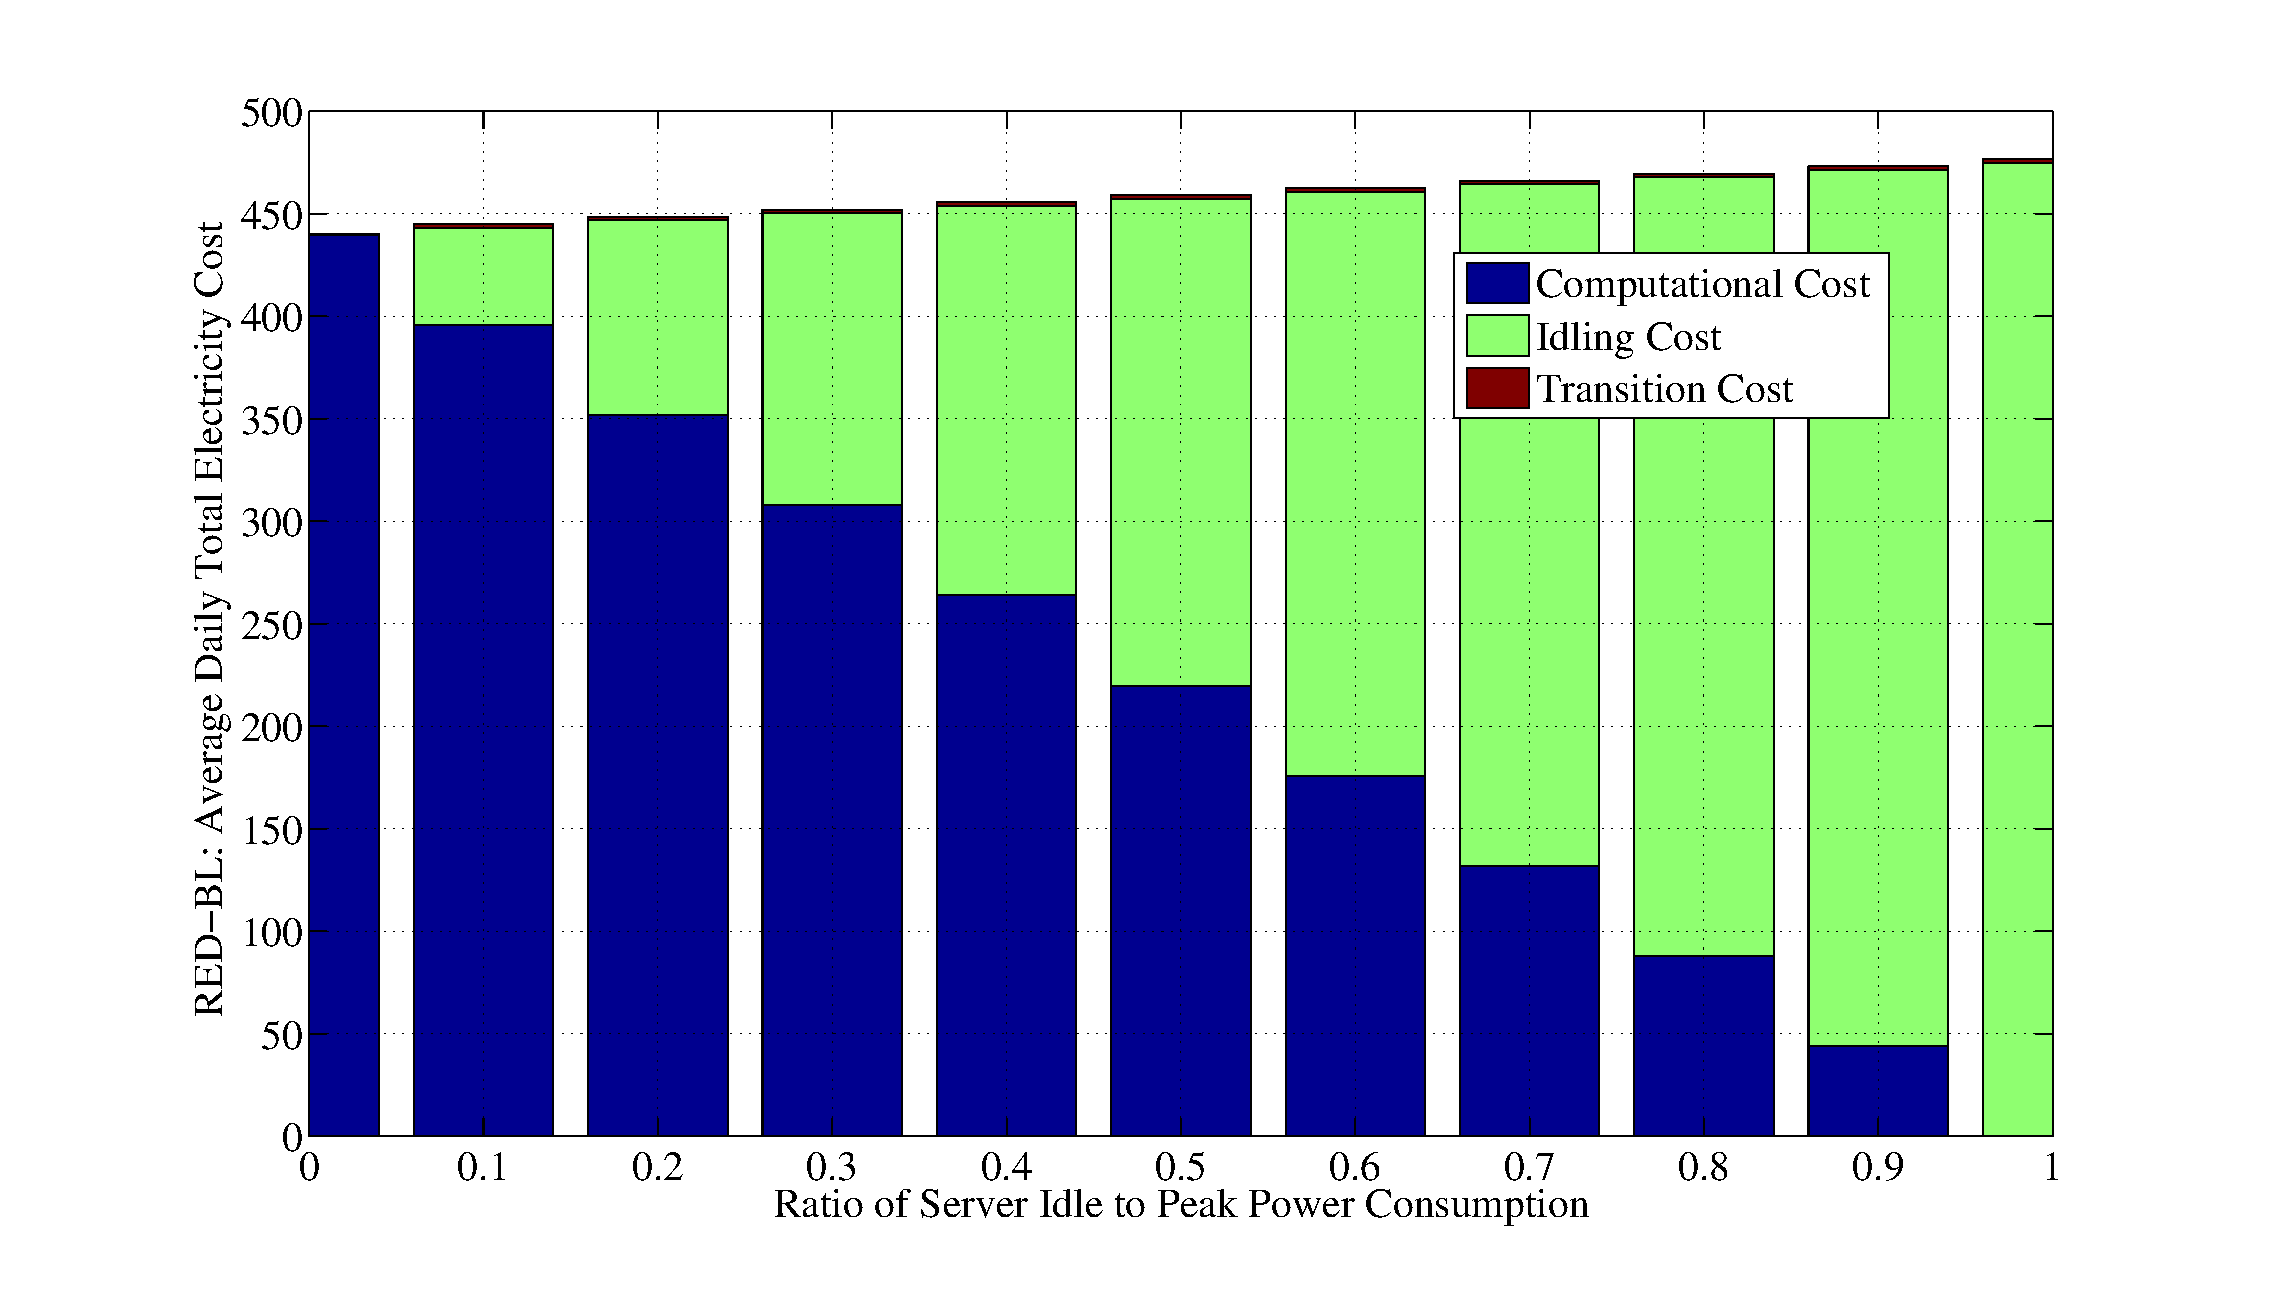
\includegraphics[width=0.8\textwidth]{pics/fvar-0.01bs.eps}
\caption{Average daily total electricity cost and it's components vs f, For b\slash s = 0.01}
\label{fig:fvar1}
\end{figure}

\begin{figure}
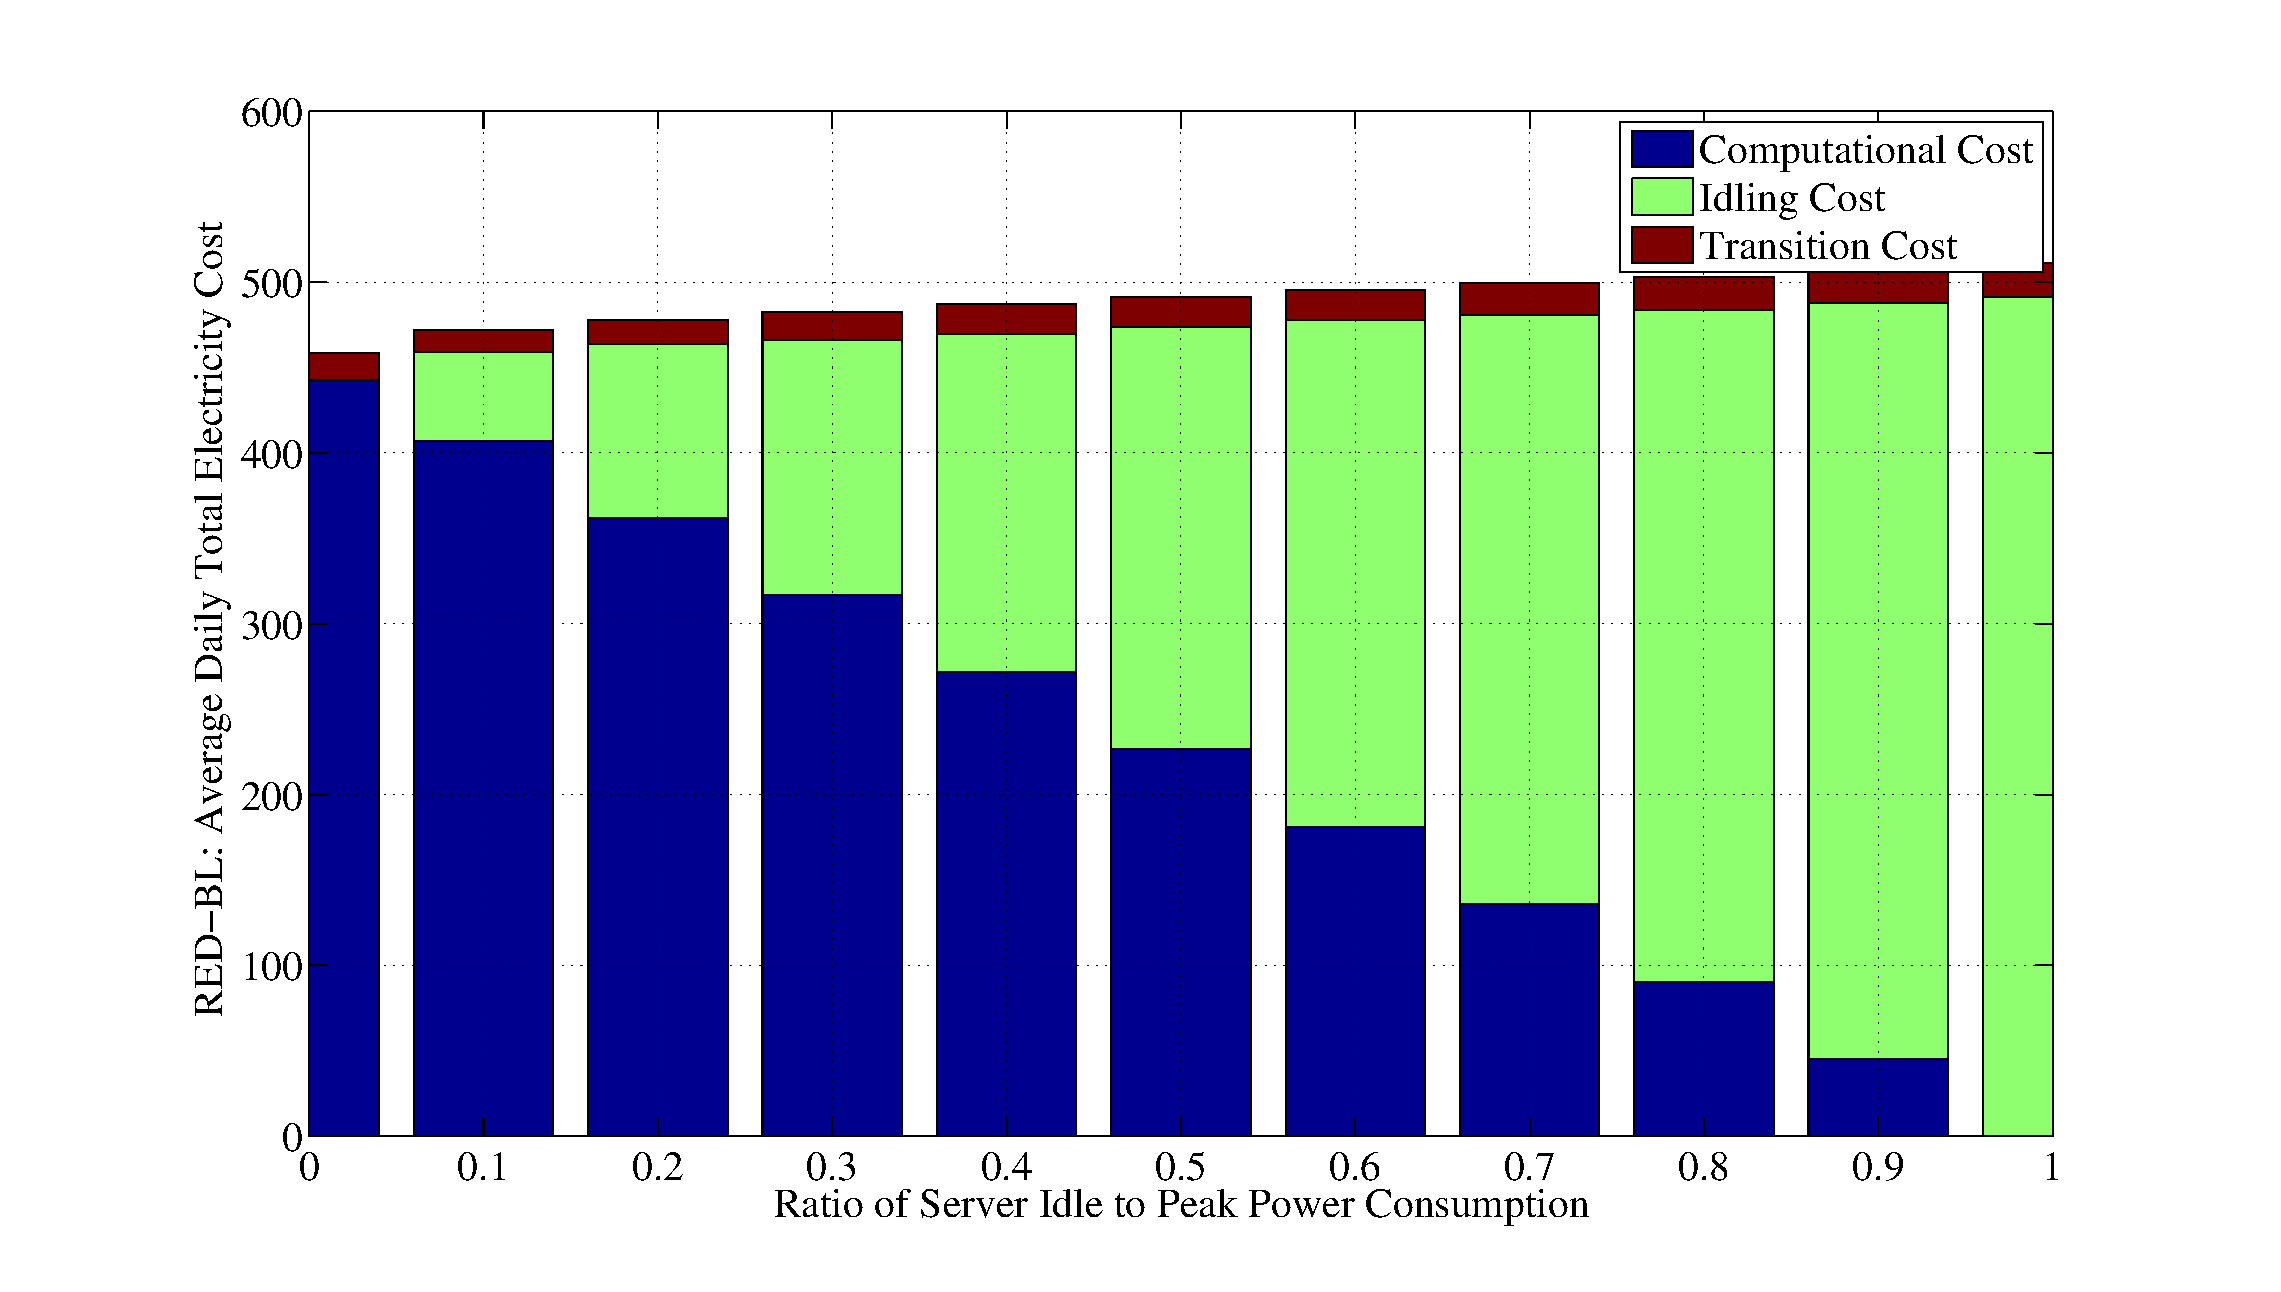
\includegraphics[width=0.8\textwidth]{pics/fvar-0.65bs.eps}
\caption{Average daily total electricity cost and it's components vs f, For b\slash s = 0.65}
\label{fig:fvar2}
\end{figure}

Figure~\ref{fig:fvar2} shows the same results for $b$/$s$=0.65. In this case, an increase from $f$=0 to $f$=1 spans an 11.44\% increase in average daily total electricity costs. Also, as $f$ drops from the typical $f$=0.65 all the way to $f$=0, the total electricity cost of the global optimal solution over the planning window drops by 7.42\%. Since the bootup/shutdown overhead is significant in this case, for all values of $f$, the total electricity cost of the global optimal solution over the planning window is characterized by an almost fixed contribution from bootup/shutdown, while the idling fraction increase almost linearly.

\subsection{Performance of the heuristic algorithm}
Figure~\ref{fig:heur1perf} shows the performance of our heuristic algorithm compared to the optimal solution of the problem for various values of the (de)activation overhead parameters. For each value of the $b$/$s$ parameters, we have plotted the average error over the seven days in our workload dataset (the curve) as well as the minimum and maximum error for any given day (the vertical bars). The performance of the heuristic is the worst for $b$/$s$ = 0, because the heuristic avoids bootup/shutdown which has zero cost for $b$/$s$ = 0. For other small values of $b$/$s$ also, the bootup/shutdown overhead is not significant and by avoiding it, our heuristic fares relatively poorly compared to the optimal solution. As the value of $b$/$s$ increases, our heuristic's error compared to the optimal solution drops until it starts a slight rise. The rising trend in the heuristic's performance for relatively high values of $b$/$s$ is because in this regime, it may often be better to allow idling of some data centers instead of a bootup at the intervals defined by $p_1$ and shutdown at those defined by $p_2$. We observed similar trends for other values of $f$ as well, when $b$/$s$ is varied from 0 to 1.

\begin{figure}
\includegraphics[width=0.8\linewidth]{pics/rb-heur1error.eps}
\caption{The minimum, maximum and average percentage difference between the cost of our heuristic and RED-BL}
\label{fig:heur1perf}
\end{figure}

\section{Summary}
In this chapter, we have instantiated the generalized problem formulation of joint workload relocation and resource pruning to optimize electricity costs for geo-diverse data centers. The generalized formulation performs a state trajectory optimization and in case of geo-diverse data centers, the network state consists of a combination of discrete as well as continuous variables. 

Our formulation determines a deployment configuration plan that is optimal over a planning window consisting of several intervals in the form of bootup/shutdown times for each data center as well as the workload to be mapped to each data center for all intervals in the planning window. Discrete optimization problems such as ours are difficult to solve exactly because of their computational complexity. However, using the CPLEX solver we were able to compute the optimal plans for planning windows consisting of 24 one-hour intervals within a few seconds. 

Our problem formulation involves several parameters whose values are expected to vary over time (for instance, the value of idle to peak power consumption ratio is expected to improve as chip and server energy proportionality improves), from one operator to another (for instance, the over provisioning ratio) and from application to application (for instance, the value of the transition cost). With so many parameters, each with many possible values, it is not possible to exhaustively test RED-BL. However, in such a case, it suffices to know the sensitivity of electricity cost savings to the variation in each parameter, while all others are held at some reasonable default values. We performed a series of such experiments for each parameter and reported the results.

Since RED-BL devises a deployment plan for a planning window based on workload forecasts, which may be somewhat erroneous, in a practical setting, RED-BL plans must be revised periodically to bring the system closer to an optimal state. For this purpose, we proposed a sliding-window re-optimization procedure and evaluated it's performance.

We used workload datasets from three live Internet applications. While the number of applications is quite small for a large geo-diverse data center operator, the statistical characteristics of the dataset are reasonably representative of such a scenario. We also used real electricity prices from 33 locations in the US that were publicly available.

While we find that RED-BL finds a useful application in electricity cost optimization of geo-diverse data centers, our thesis is not the final word on this problem. Several avenues of further exploration are yet to be explored. We have listed some future work in Chapter~\ref{chap:conclusions}.